% I-ITSM project report. Build with XeLaTeX (needed for the Cambria / Calibri fonts):
%     cd docs/report/latex && xelatex report.tex && xelatex report.tex
% Edit the group details in the "Group details" block below before submitting.
\documentclass[11pt,a4paper]{article}

% ------------------------------------------------------------------ fonts
\usepackage{amsmath}
\usepackage{fontspec}
% Headings in Cambria, text in Calibri. On machines without the Microsoft fonts
% (e.g. Linux) the metric-compatible Caladea / Carlito are used instead.
\IfFontExistsTF{Calibri}{\setmainfont{Calibri}}{\setmainfont{Carlito}}
\IfFontExistsTF{Cambria}{\newfontfamily\headingfont{Cambria}}{\newfontfamily\headingfont{Caladea}}
\IfFontExistsTF{Consolas}{\setmonofont{Consolas}[Scale=0.88]}{\setmonofont{DejaVu Sans Mono}[Scale=0.82]}

% ------------------------------------------------------------------ layout
\usepackage[a4paper,top=2.3cm,bottom=2.3cm,left=2.3cm,right=2.3cm,headheight=14pt]{geometry}
\usepackage{xcolor}
\definecolor{brand}{HTML}{3730A3}
\definecolor{brand2}{HTML}{6D28D9}
\definecolor{ink}{HTML}{1F2937}
\definecolor{muted}{HTML}{5B6472}
\definecolor{rowtint}{HTML}{F3F4FB}
\color{ink}
\usepackage{graphicx}
\usepackage{float}
\usepackage{array,tabularx,longtable,booktabs}
\usepackage[table]{xcolor}
\usepackage{enumitem}
\usepackage{caption}
\usepackage{subcaption}
\usepackage{pdflscape}
\usepackage{fancyhdr}
\usepackage{titlesec}
\usepackage[hidelinks]{hyperref}
\hypersetup{colorlinks=true,linkcolor=brand,urlcolor=brand2,citecolor=brand}

\setlength{\parindent}{0pt}
\setlength{\parskip}{0.55em}
\linespread{1.08}
\setlist{itemsep=0.15em,topsep=0.3em,parsep=0pt}
\renewcommand{\arraystretch}{1.25}
\setlength{\tabcolsep}{5pt}

\titleformat{\section}{\headingfont\LARGE\bfseries\color{brand}}{\thesection}{0.6em}{}
\titleformat{\subsection}{\headingfont\Large\bfseries\color{brand}}{\thesubsection}{0.6em}{}
\titleformat{\subsubsection}{\headingfont\large\bfseries\color{ink}}{\thesubsubsection}{0.6em}{}
\titlespacing*{\section}{0pt}{1.2em}{0.5em}
\titlespacing*{\subsection}{0pt}{1em}{0.35em}
\titlespacing*{\subsubsection}{0pt}{0.8em}{0.25em}

\captionsetup{font={small,color=muted},labelfont={bf,color=brand},skip=5pt}

\pagestyle{fancy}
\fancyhf{}
\renewcommand{\headrulewidth}{0pt}
\fancyhead[L]{\small\color{muted}I-ITSM: Intelligent IT Service Management}
\fancyhead[R]{\small\color{muted}CS F213 Object-Oriented Programming}
\fancyfoot[C]{\small\color{muted}\thepage}

\newcommand{\code}[1]{\texttt{\hyphenchar\font=`\-\relax #1}}
\usepackage{needspace}
\newcommand{\shot}[2]{\begin{figure}[H]\centering\includegraphics[width=\linewidth]{figures/shot-#1.jpg}\caption{#2}\end{figure}}
\newcommand{\twoshots}[4]{%
\begin{figure}[H]\centering
\begin{subfigure}[t]{0.495\linewidth}\includegraphics[width=\linewidth]{figures/shot-#1.jpg}\caption{#2}\end{subfigure}\hfill
\begin{subfigure}[t]{0.495\linewidth}\includegraphics[width=\linewidth]{figures/shot-#3.jpg}\caption{#4}\end{subfigure}
\end{figure}}
\newcolumntype{L}[1]{>{\raggedright\arraybackslash}p{#1}}
\newcolumntype{Y}{>{\raggedright\arraybackslash}X}

% ------------------------------------------------------------------ code listings
\usepackage{listings}
\definecolor{codebg}{HTML}{F6F7FB}
\definecolor{codekw}{HTML}{4338CA}
\definecolor{codecm}{HTML}{6B7280}
\definecolor{codestr}{HTML}{047857}
\lstdefinestyle{java}{language=Java,basicstyle=\ttfamily\footnotesize,keywordstyle=\color{codekw}\bfseries,
  commentstyle=\color{codecm}\itshape,stringstyle=\color{codestr},backgroundcolor=\color{codebg},
  frame=leftline,framerule=2pt,rulecolor=\color{brand},xleftmargin=6pt,framexleftmargin=6pt,
  showstringspaces=false,columns=fullflexible,keepspaces=true,breaklines=true,tabsize=4,
  aboveskip=0.6em,belowskip=0.4em,morekeywords={record,var,sealed,permits}}
\lstset{style=java}
\renewcommand{\lstlistingname}{Listing}

% ------------------------------------------------------------------ group details (edit these)
\newcommand{\groupno}{12}
\newcommand{\repourl}{https://github.com/VijaySrivathsan/I-ITSM}
\newcommand{\videoname}{\groupno\_OOP\_S1\_2025-2026\_Project}

\begin{document}

% ================================================================== title page
\begin{titlepage}
\thispagestyle{empty}
\vspace*{2.2cm}
{\headingfont\color{muted}\large CS F213 / MAC F212 Object-Oriented Programming\par}
{\headingfont\color{muted}\large Semester I, 2026--2027\par}
\vspace{1.6cm}
{\headingfont\bfseries\color{brand}\fontsize{34}{40}\selectfont I-ITSM\par}
\vspace{0.4cm}
{\headingfont\color{brand2}\LARGE Intelligent IT Service Management\\[0.2em] \& Incident Resolution System\par}
\vspace{0.8cm}
{\Large Project Report\par}
\vspace{1.8cm}
{\large
\begin{tabular}{@{}L{3.6cm}L{10cm}@{}}
\textbf{Group} & Group \groupno \\
\textbf{Members} & Vijay Srivathsan B \hfill 2024B3A70537H \\
 & Sathvik T Hatwar \hfill 2024B3A70509H \\
 & Harish MP \hfill 2024B5A70641H \\
 & Vishnu Rahul \hfill 2024B4AD0542H \\
\textbf{Repository} & \url{\repourl} \\
\textbf{Demo video} & \videoname \\
\end{tabular}\par}
\vfill
{\color{muted}A web application that manages the complete life of an IT incident: report, classify, prioritise, assign, investigate, resolve, verify and close. Built with Java 21 and Spring Boot, designed around object-oriented principles and seven design patterns.\par}
\end{titlepage}

\setcounter{tocdepth}{1}
\tableofcontents
\clearpage

% ================================================================== 1
\section{Problem Analysis}

\subsection{Problem}
Modern organisations depend on IT services such as payment applications, databases, networks, authentication and storage. When one of them fails, the problem is often reported by email, phone or spreadsheet. In a large organisation, with hundreds of incidents a day, this leads to:
\begin{itemize}
  \item urgent problems waiting behind trivial ones, because nobody calculates priority consistently;
  \item the same outage being reported many times by different people;
  \item technicians who are overloaded while others are idle;
  \item deadlines (SLAs) that are missed without anyone noticing in time;
  \item no reliable record of who did what, and no view of recurring problems.
\end{itemize}

\subsection{Stakeholders}
\begin{tabularx}{\linewidth}{@{}L{4.2cm}Y@{}}
\toprule
\textbf{Stakeholder} & \textbf{Needs} \\
\midrule
Employees / customers & Report a problem quickly, follow its progress, answer questions, confirm the fix. \\
Technicians & A clear queue ordered by urgency, a fair workload, and the history needed to investigate. \\
Team leads & Visibility of the team's workload and of critical incidents that nobody has picked up. \\
Administrators / IT managers & Configuration (services, categories, SLAs, strategies), compliance figures, reports and an audit trail. \\
\bottomrule
\end{tabularx}

\subsection{Proposed solution}
I-ITSM is a role-based web application that manages the whole incident lifecycle:
\textit{Report $\rightarrow$ Classify $\rightarrow$ Prioritise $\rightarrow$ Assign $\rightarrow$ Investigate $\rightarrow$ Resolve $\rightarrow$ Verify $\rightarrow$ Close}. It
\begin{itemize}
  \item calculates priority automatically from impact, urgency, business criticality and the number of affected users, and shows the working;
  \item assigns technicians with an interchangeable strategy (skill, load, round-robin or a scored recommendation);
  \item monitors SLA deadlines in the background, warns before a breach and escalates unacknowledged critical incidents;
  \item notifies people through in-app, e-mail and SMS channels, and records every action in an audit trail;
  \item detects duplicate and related reports, suggests categories and past resolutions, and offers an AI root-cause advisor;
  \item gives administrators search, dashboards, CSV export and configuration screens.
\end{itemize}

\subsection{Assumptions}
\begin{itemize}
  \item One organisation; employees self-register, administrators create technicians and other administrators.
  \item E-mail and SMS are simulated (allowed by the brief); messages go to an outbox that administrators can inspect.
  \item Times are stored in UTC and shown in Asia/Kolkata time.
  \item The SLA clock keeps running while the incident waits for the reporter (a stated simplification).
  \item The brief's SLA targets are the defaults (P1 5 min / 30 min, P2 15 min / 2 h, P3 1 h / 8 h, P4 4 h / 24 h); administrators can override them per service.
\end{itemize}

% ================================================================== 2
\section{Requirements Specification}

\subsection{Functional requirements}
\begin{longtable}{@{}L{1.1cm}L{8.6cm}L{5.4cm}@{}}
\toprule
\textbf{ID} & \textbf{Requirement} & \textbf{Implemented in} \\
\midrule\endhead
FR1 & Employees register; all users log in; three roles: Employee, Technician, Administrator & \code{AuthController}, \code{UserService}, \code{SecurityConfig} \\
FR2 & Employees report incidents (service, optional category, title, description, impact, urgency, affected users) & \code{EmployeeController}, \code{IncidentFactory} \\
FR3 & The system classifies incidents and calculates priority P1--P4 & \code{PriorityService}, \code{WeightedScoring\-PriorityStrategy} \\
FR4 & The applicable SLA is found (service-specific or default); response and resolution deadlines are tracked & \code{SlaService}, \code{SlaRecord} \\
FR5 & A technician is assigned with a configurable strategy; administrators can reassign & \code{AssignmentService}, \code{AssignmentStrategy\-Registry} \\
FR6 & Technicians acknowledge, investigate, request information and resolve; reporters answer, verify, reopen and close & \code{IncidentService}, \code{IncidentController} \\
FR7 & Illegal lifecycle transitions are rejected & State pattern, \code{domain.incident.state} \\
FR8 & Relevant people are notified of important events (in-app, e-mail, SMS) & \code{NotificationListener}, channels, gateways \\
FR9 & Every action is recorded: time, user, action, incident, previous and new state, description & \code{AuditListener}, \code{AuditService} \\
FR10 & Search with ten combinable criteria; CSV export & \code{SearchService}, \code{IncidentSpecifications} \\
FR11 & Dashboard: totals, open, critical, resolved, SLA violations, compliance, workload, breakdowns & \code{ReportService} \\
FR12 & Background SLA monitoring with warnings and violation recording & \code{SlaMonitor}, \code{SlaMonitorService} \\
FR13 & Intelligent features A--G, AI advisor and service dependency impact (Section~\ref{sec:intelligent}) & \code{intelligence} package \\
FR14 & Administrators manage users, technicians, services, categories, SLA policies and the assignment strategy & \code{AdminController}, \code{CatalogService} \\
\bottomrule
\end{longtable}

\subsection{Non-functional requirements}
\begin{tabularx}{\linewidth}{@{}L{3.4cm}Y@{}}
\toprule
\textbf{Quality} & \textbf{How it is met} \\
\midrule
Maintainability & Categories are data, not code. A new priority algorithm, assignment strategy, notification channel or risk rule is one new class (open--closed principle). \\
Security & Authentication, role-based authorisation in three layers, BCrypt passwords, CSRF tokens, validation, ownership checks (Section~\ref{sec:security}). \\
Reliability & An incident change and its audit line commit in one transaction; a failing SMS provider never blocks an update; optimistic locking prevents lost updates. \\
Usability & A different home page per role; only currently allowed actions are shown; SLA countdowns; light and dark themes; keyboard access; works at phone width. \\
Testability & A \code{Clock} is injected everywhere, so time rules are tested without waiting; 249 automated tests. \\
Portability & H2 for tests and development, PostgreSQL for the demo; JPA keeps the code database-independent. Front-end libraries are bundled, so the UI works offline. \\
\bottomrule
\end{tabularx}

\subsection{User roles}
\begin{tabularx}{\linewidth}{@{}L{3cm}Y@{}}
\toprule
\textbf{Role} & \textbf{Can} \\
\midrule
Employee & Register, report, track own incidents, add information, answer requests, verify with feedback, reopen, close, search own incidents. \\
Technician & View the queue (most urgent SLA first) and workload, set availability, acknowledge, investigate, add notes, request information, resolve, confirm or dismiss duplicates. \\
Team lead & Everything a technician can, plus all incidents and team workload; first level of escalation. \\
Administrator & Manage users, technicians, services, categories, SLA policies and the strategy; classify and assign; dashboard, audit log, outbox, CSV export. \\
\bottomrule
\end{tabularx}

\subsection{Business rules}
\begin{enumerate}
  \item Priority is always calculated, never typed in: score $=$ impact (1--3) $\times$ urgency (1--3) $\times$ criticality (1--5) $\times$ user factor (1.0 / 1.2 / 1.5 / 2.0). P1 if score $\geq 30$, P2 $\geq 15$, P3 $\geq 6$, otherwise P4.
  \item SLA deadlines run from the time of reporting. Meeting a deadline exactly is not a breach; a breach is permanent and reported once.
  \item A technician never receives an incident while unavailable or at maximum workload; if nobody is eligible, administrators are alerted.
  \item Only the assigned technician acknowledges, works on and resolves an incident; only the reporter answers, reopens or gives feedback.
  \item An unacknowledged P1/P2 escalates to the team lead, then the system administrator, then the IT manager, one response window apart.
  \item An employee cannot file the same report again within one hour; similar reports from others are flagged for a person to confirm.
  \item Nobody is notified about their own action; SMS is used only for urgent events.
\end{enumerate}

% ================================================================== 3
\clearpage
\section{System Architecture}
The application is a layered Spring Boot application. Each layer depends only on the layer below it, and side effects such as auditing and notifications are triggered through domain events rather than direct calls.

\begin{figure}[H]\centering
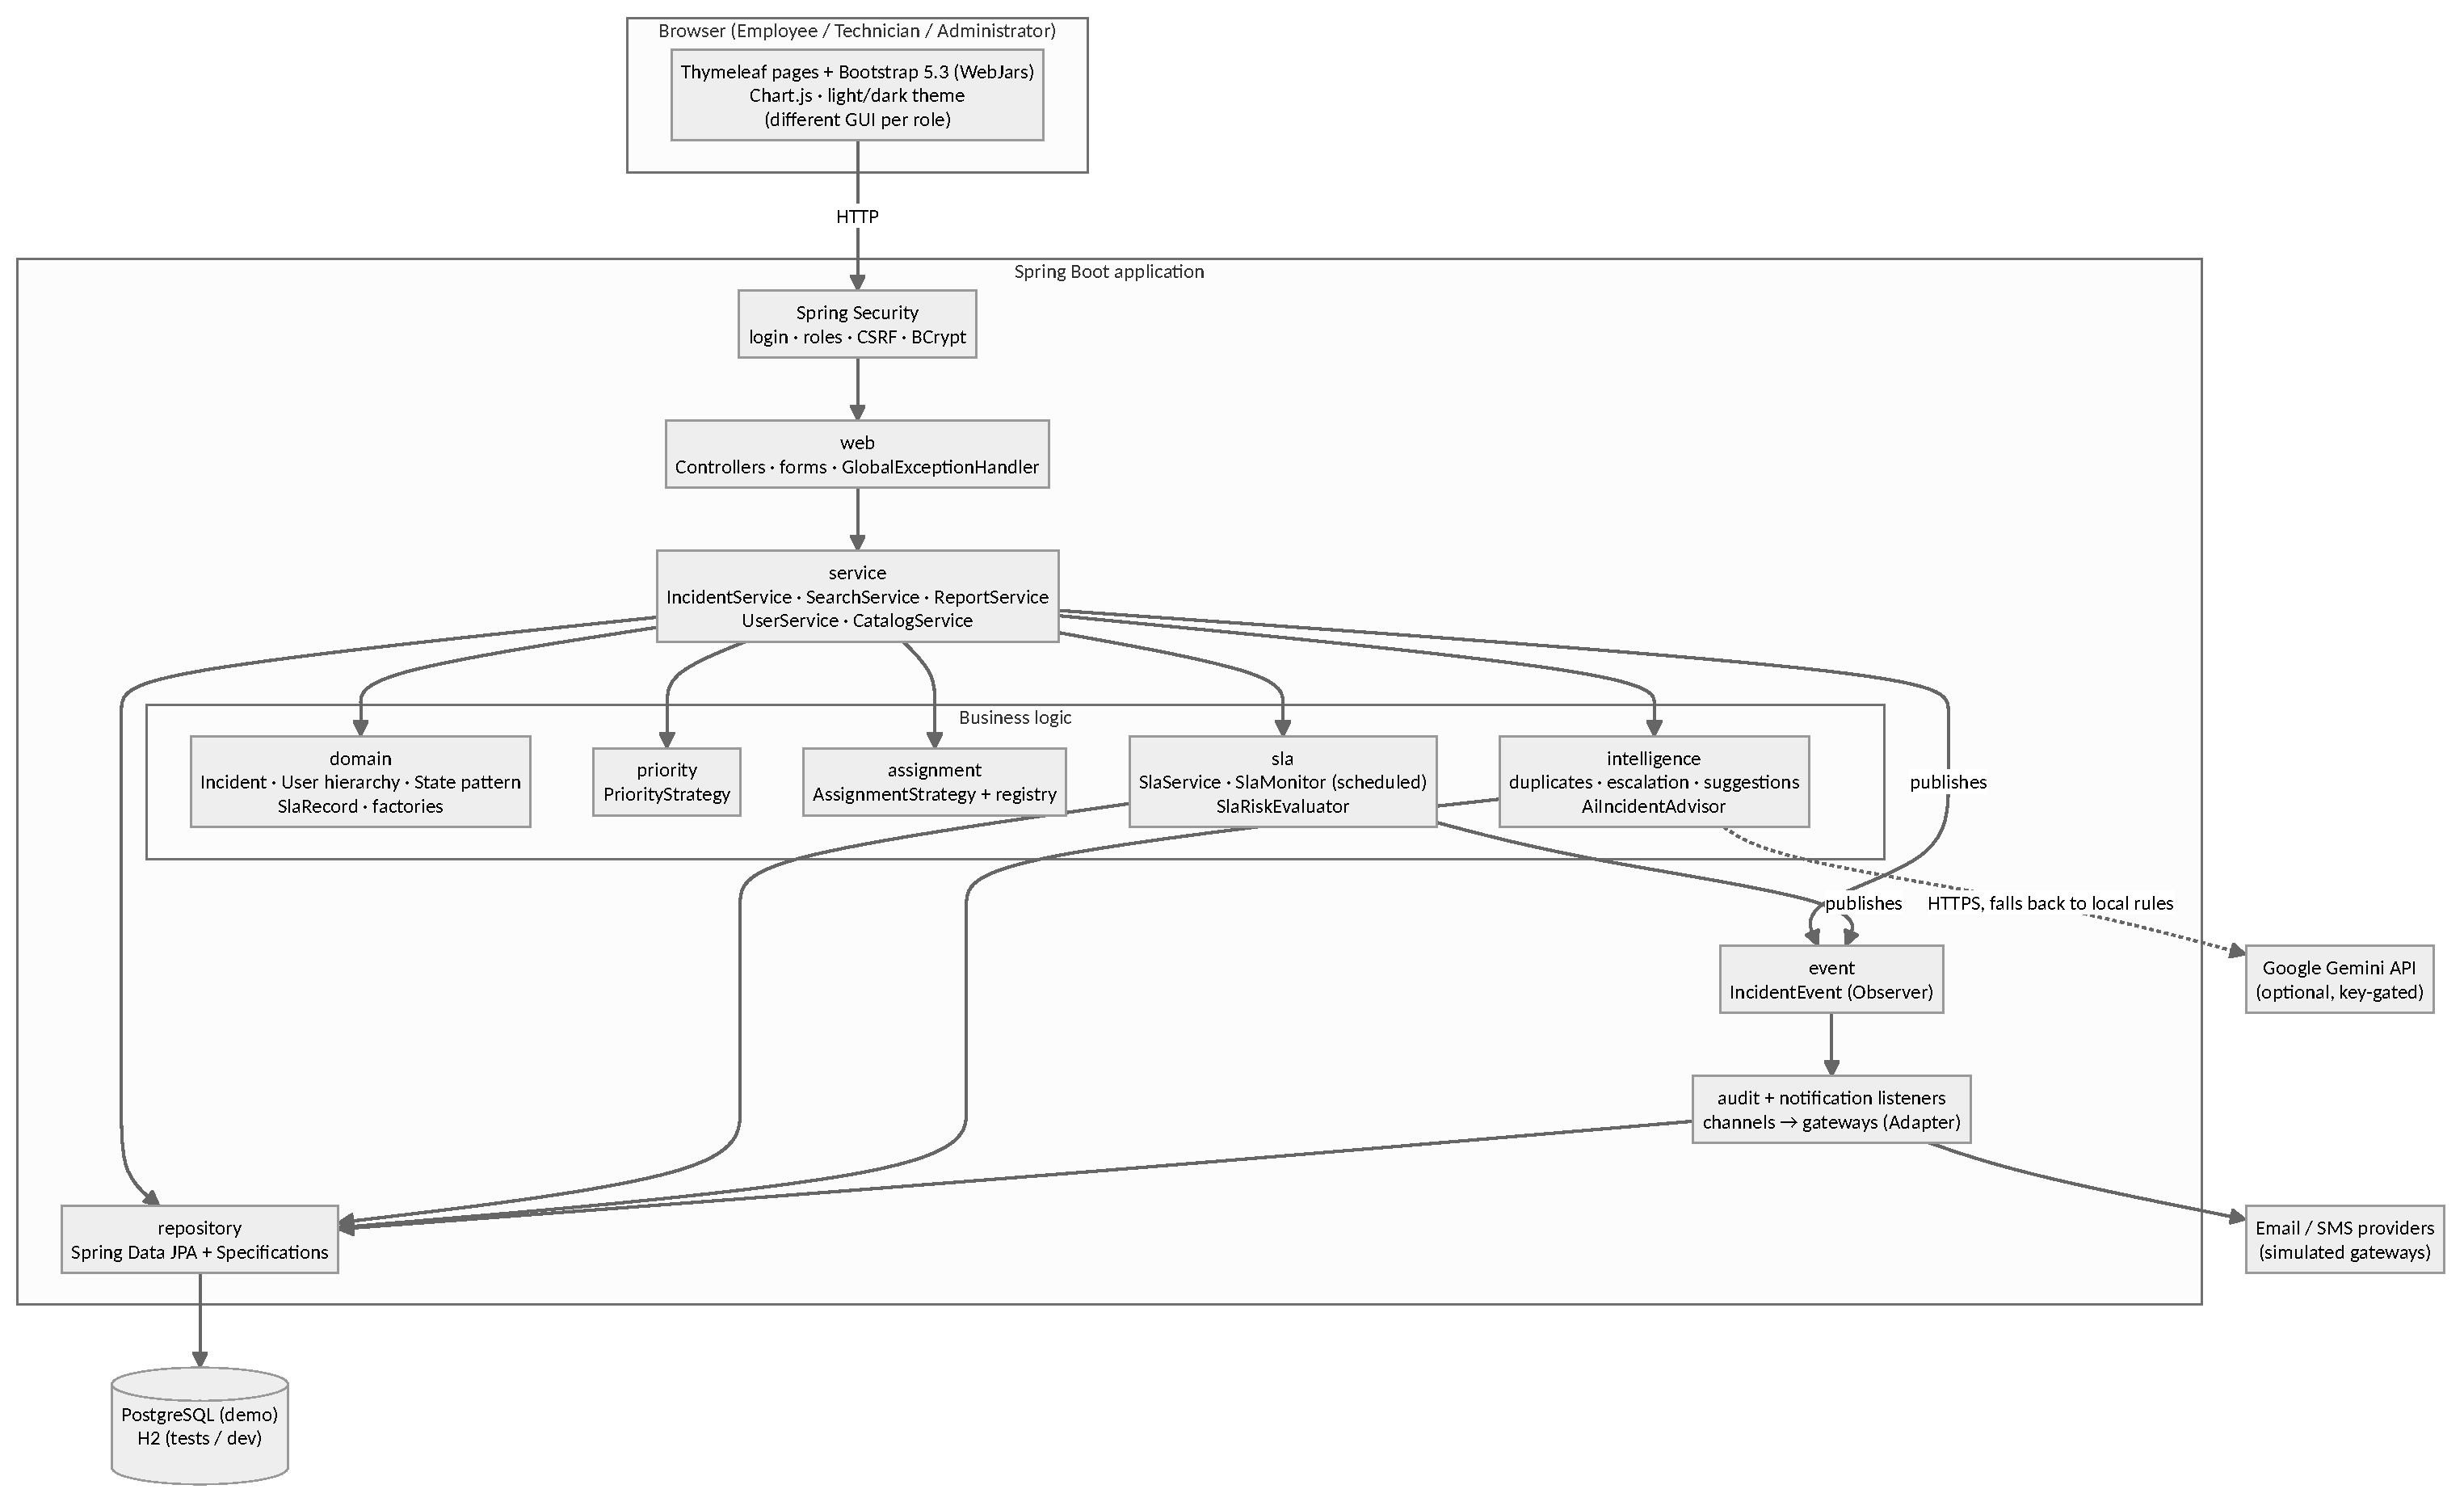
\includegraphics[width=\linewidth]{figures/architecture.pdf}
\caption{Layered architecture and the main components}
\end{figure}

\begin{tabularx}{\linewidth}{@{}L{3.2cm}Y@{}}
\toprule
\textbf{Package} & \textbf{Responsibility} \\
\midrule
\code{web} & Controllers, form objects, one \code{GlobalExceptionHandler}. Controllers only call services. \\
\code{service} & Use cases: reporting, lifecycle actions, search, reports, catalogue, users. \\
\code{domain} & Entities and value objects (\code{Incident}, \code{User} hierarchy, \code{SlaRecord}), the State pattern and factories. Domain objects enforce their own rules. \\
\code{priority}, \code{assignment} & Strategy interfaces and their implementations. \\
\code{sla}, \code{intelligence} & SLA calculation and background monitor; duplicates, escalation, suggestions, AI advisor. \\
\code{event}, \code{audit}, \code{notification} & Domain events (Observer), audit listener, notification channels and gateway adapters. \\
\code{repository} & Spring Data JPA repositories and search specifications. \\
\bottomrule
\end{tabularx}

Why a layered monolith: it is the simplest structure that still separates presentation, business logic and persistence; every class is easy to explain and test; and the event bus and strategy interfaces mark exactly where the system could later be split into services.

% ================================================================== 4
\needspace{6\baselineskip}
\section{UML Diagrams and Object-Oriented Design}

\subsection{Use case diagram}
\begin{figure}[H]\centering
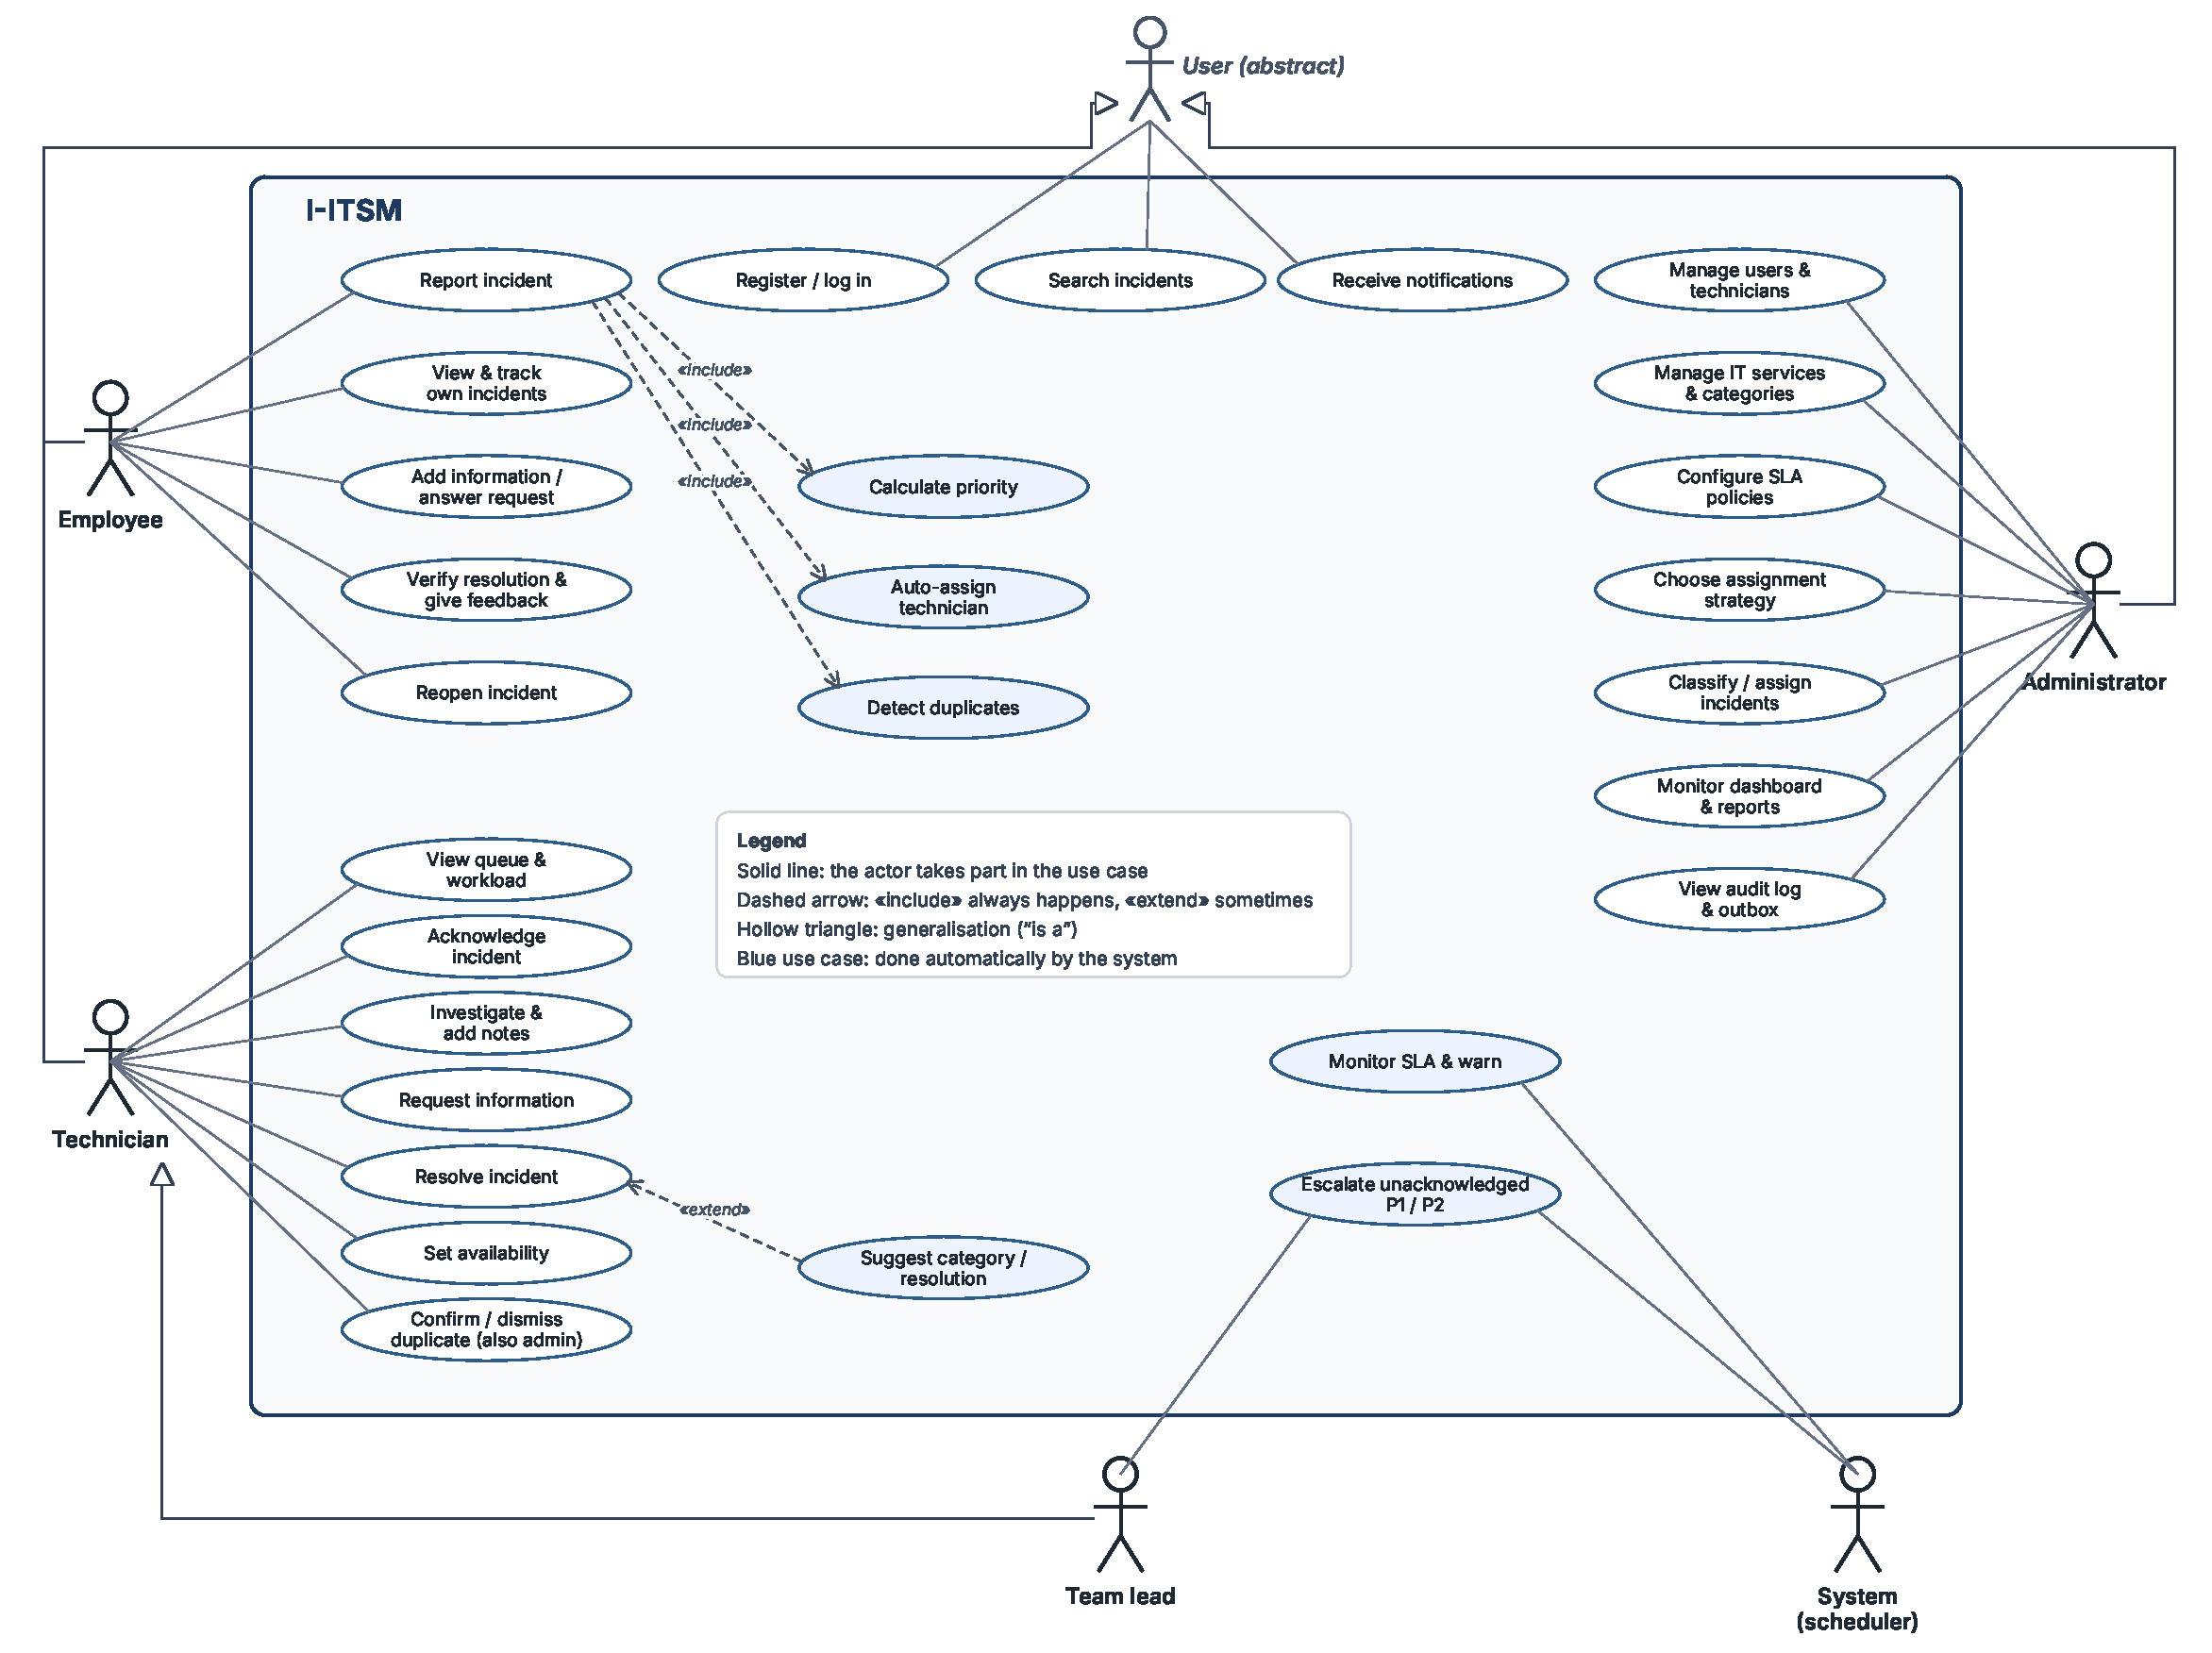
\includegraphics[width=\linewidth]{figures/use-case.pdf}
\caption{Use cases. Employee, Technician and Administrator specialise an abstract User; a team lead is a technician. Blue use cases are performed automatically.}
\end{figure}

\subsection{Object-oriented concepts in the code}
\begin{longtable}{@{}L{3.1cm}L{12.1cm}@{}}
\toprule
\textbf{Concept} & \textbf{Where it appears} \\
\midrule\endhead
Encapsulation & \code{Incident} has no public setters; its state changes only through intent-revealing methods (\code{assignTo}, \code{resolve}, \code{reopen}). Collections are returned as read-only views; constructors validate their arguments. \\
Abstraction & Interfaces \code{IncidentState}, \code{PriorityStrategy}, \code{AssignmentStrategy}, \code{NotificationChannel}, \code{DuplicateDetector}, \code{SlaRiskEvaluator}: callers depend on what is done, not how. \\
Inheritance (true is-a) & \code{User} $\rightarrow$ \code{Employee}, \code{Technician}, \code{Administrator}; \code{AbstractIncidentState} $\rightarrow$ 9 states; \code{ItsmException} $\rightarrow$ exception families; \code{BaseEntity} $\rightarrow$ entities. \\
Polymorphism & \code{incident.resolve()} behaves differently in each state; \code{user.getRole()}; the same input gives P1 with the weighted strategy and P3 with the matrix strategy (tested). \\
Interfaces & 20 contracts, including the gateways \code{EmailGateway} and \code{SmsGateway}. \\
Composition & \code{Incident} owns its \code{SlaRecord}, \code{Resolution}, \code{Feedback} and \code{InvestigationNote}s (they live and die with it). \\
Association / aggregation & An incident refers to its reporter, assignee, service and category; technicians share \code{Category} objects as skills; services depend on other services. \\
Exceptions & One hierarchy under \code{ItsmException}, handled in one \code{@ControllerAdvice} (Section~\ref{sec:security}). \\
Collections & \code{EnumMap} (state registry, priority matrix), \code{PriorityQueue} (load-based assignment), \code{ConcurrentHashMap} with \code{AtomicInteger} (round-robin), \code{Deque} (escalation chain), \code{LinkedHashMap} (ordered reports), \code{Set} (skills, word sets for similarity). \\
\bottomrule
\end{longtable}

\begin{landscape}
\subsection{Class diagram: domain model}
\begin{figure}[H]\centering
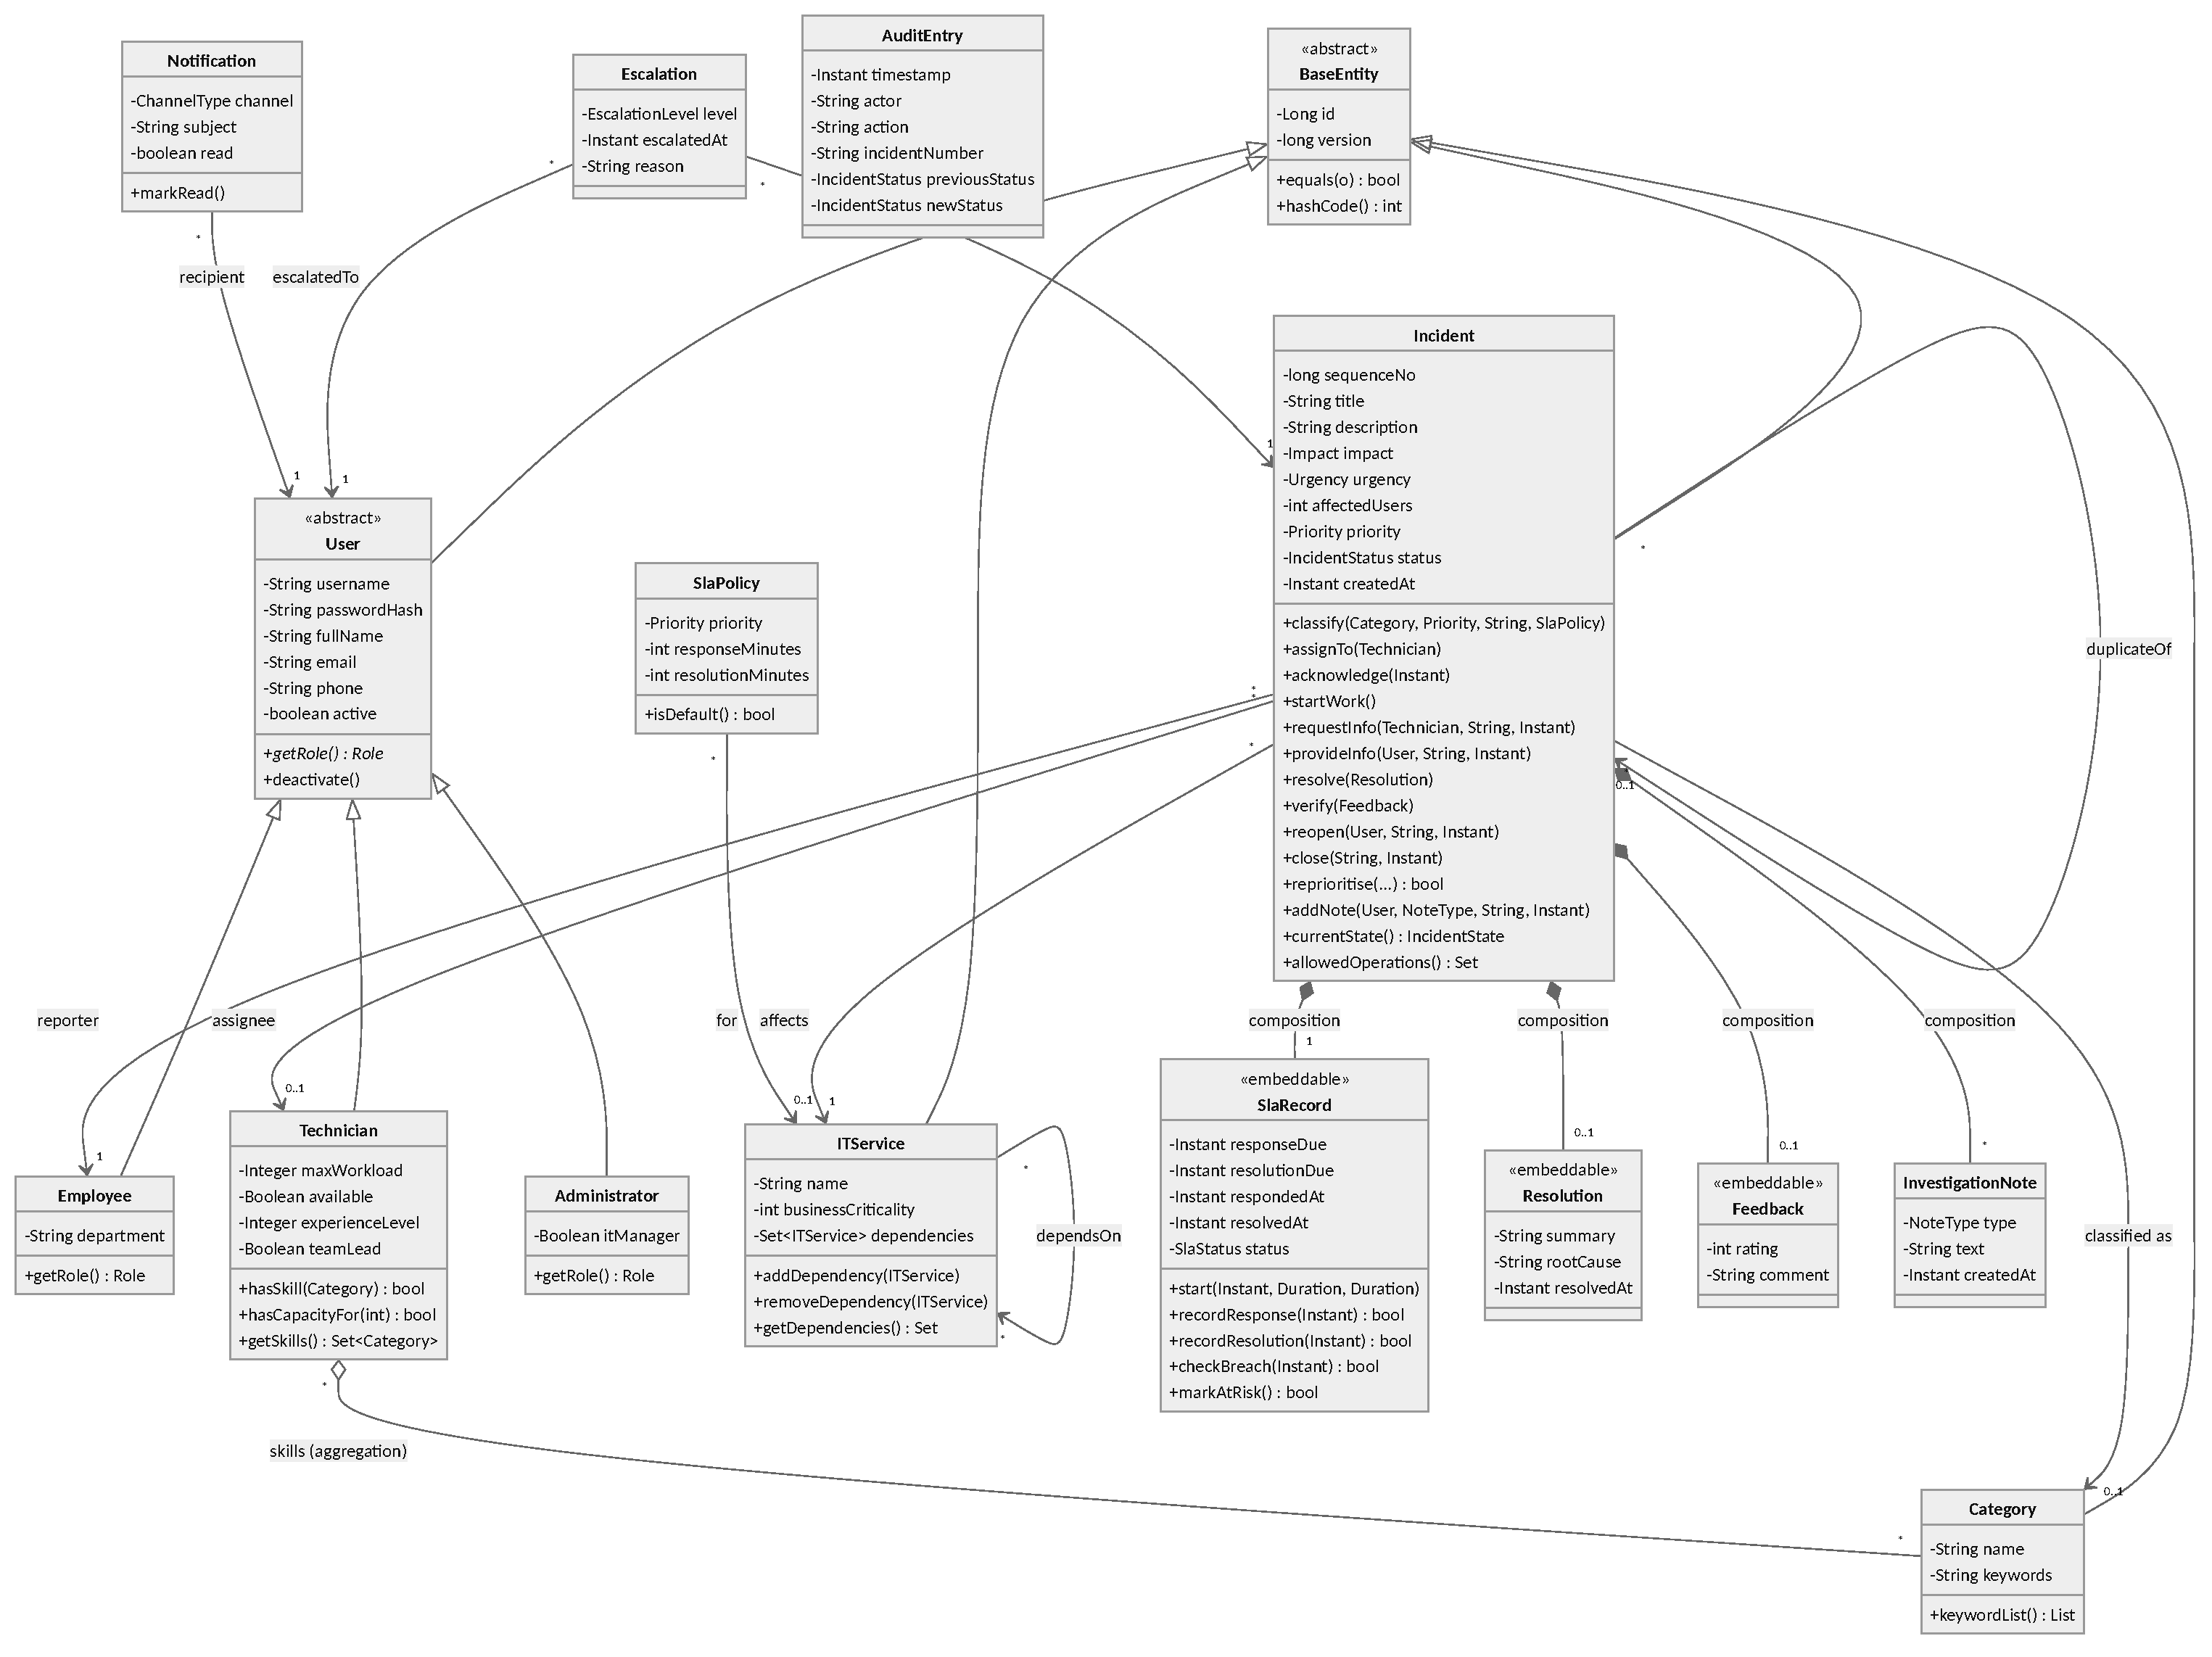
\includegraphics[height=0.84\textheight,width=\linewidth,keepaspectratio]{figures/domain-class.pdf}
\caption{Domain model: classes, attributes, methods, inheritance (\code{User} $\rightarrow$ \code{Employee} / \code{Technician} / \code{Administrator}), associations, composition (\code{Incident} owns \code{SlaRecord}, \code{Resolution}, \code{Feedback}, notes) and aggregation (technician skills).}
\end{figure}
\end{landscape}

\subsection{Class diagrams: design patterns}
\begin{figure}[H]\centering
\begin{subfigure}[t]{0.56\linewidth}\centering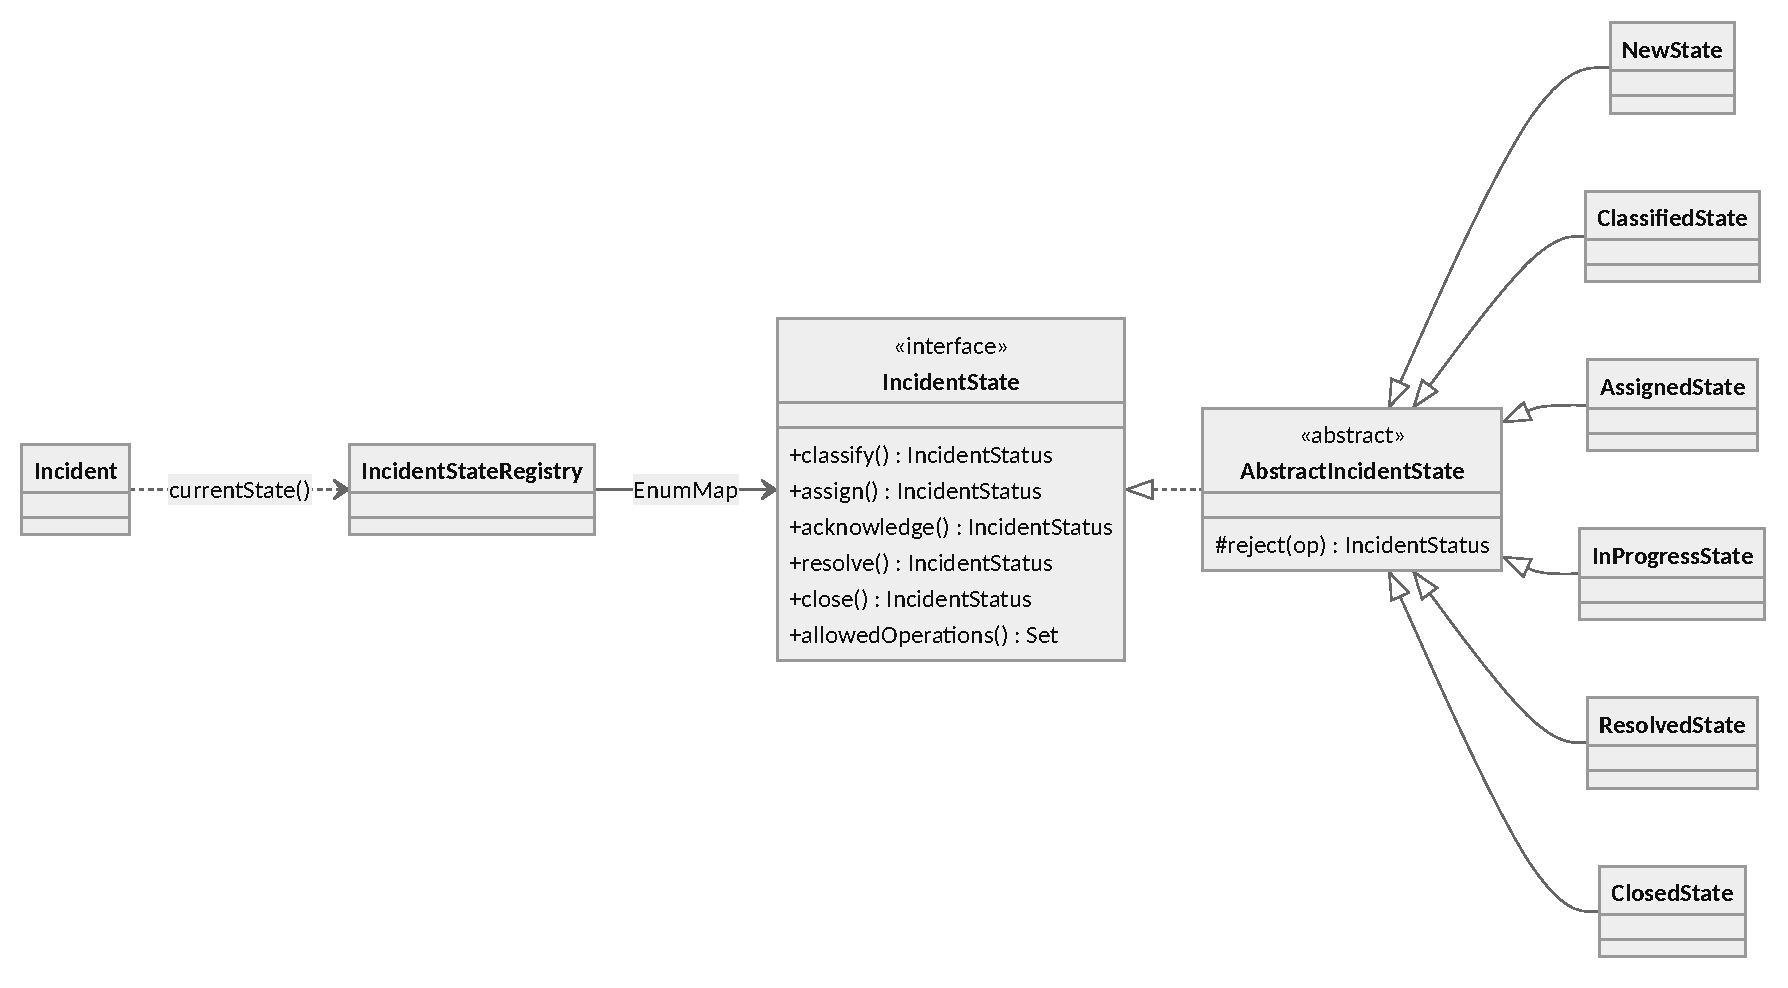
\includegraphics[width=\linewidth]{figures/pattern-state.pdf}\caption{State: one class per incident status}\end{subfigure}\hfill
\begin{subfigure}[t]{0.42\linewidth}\centering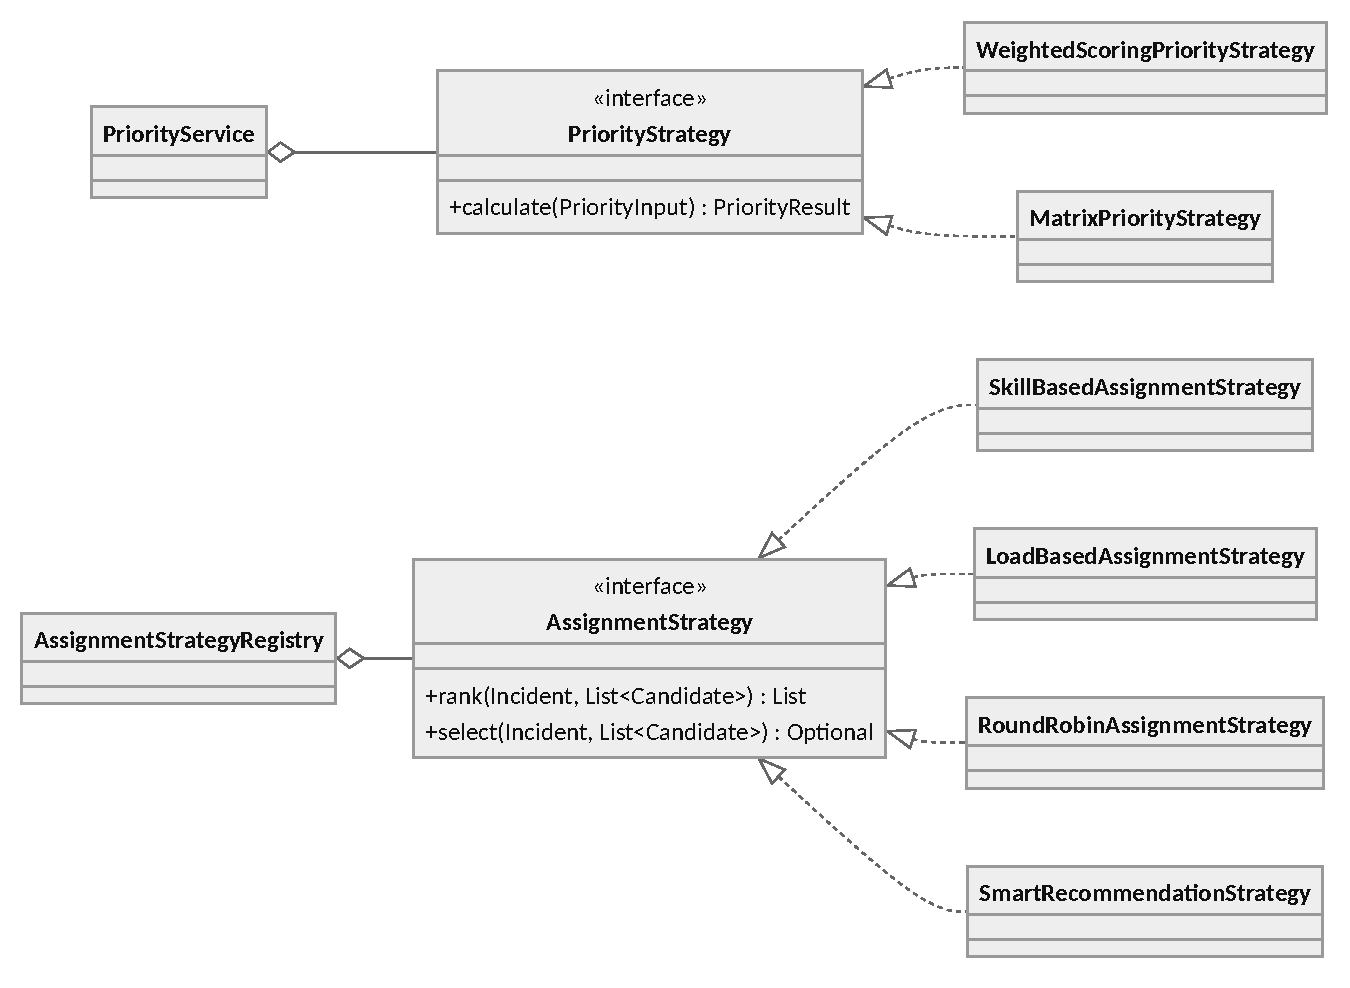
\includegraphics[width=\linewidth]{figures/pattern-strategy.pdf}\caption{Strategy: priority and assignment}\end{subfigure}
\par\medskip
\begin{subfigure}[t]{\linewidth}\centering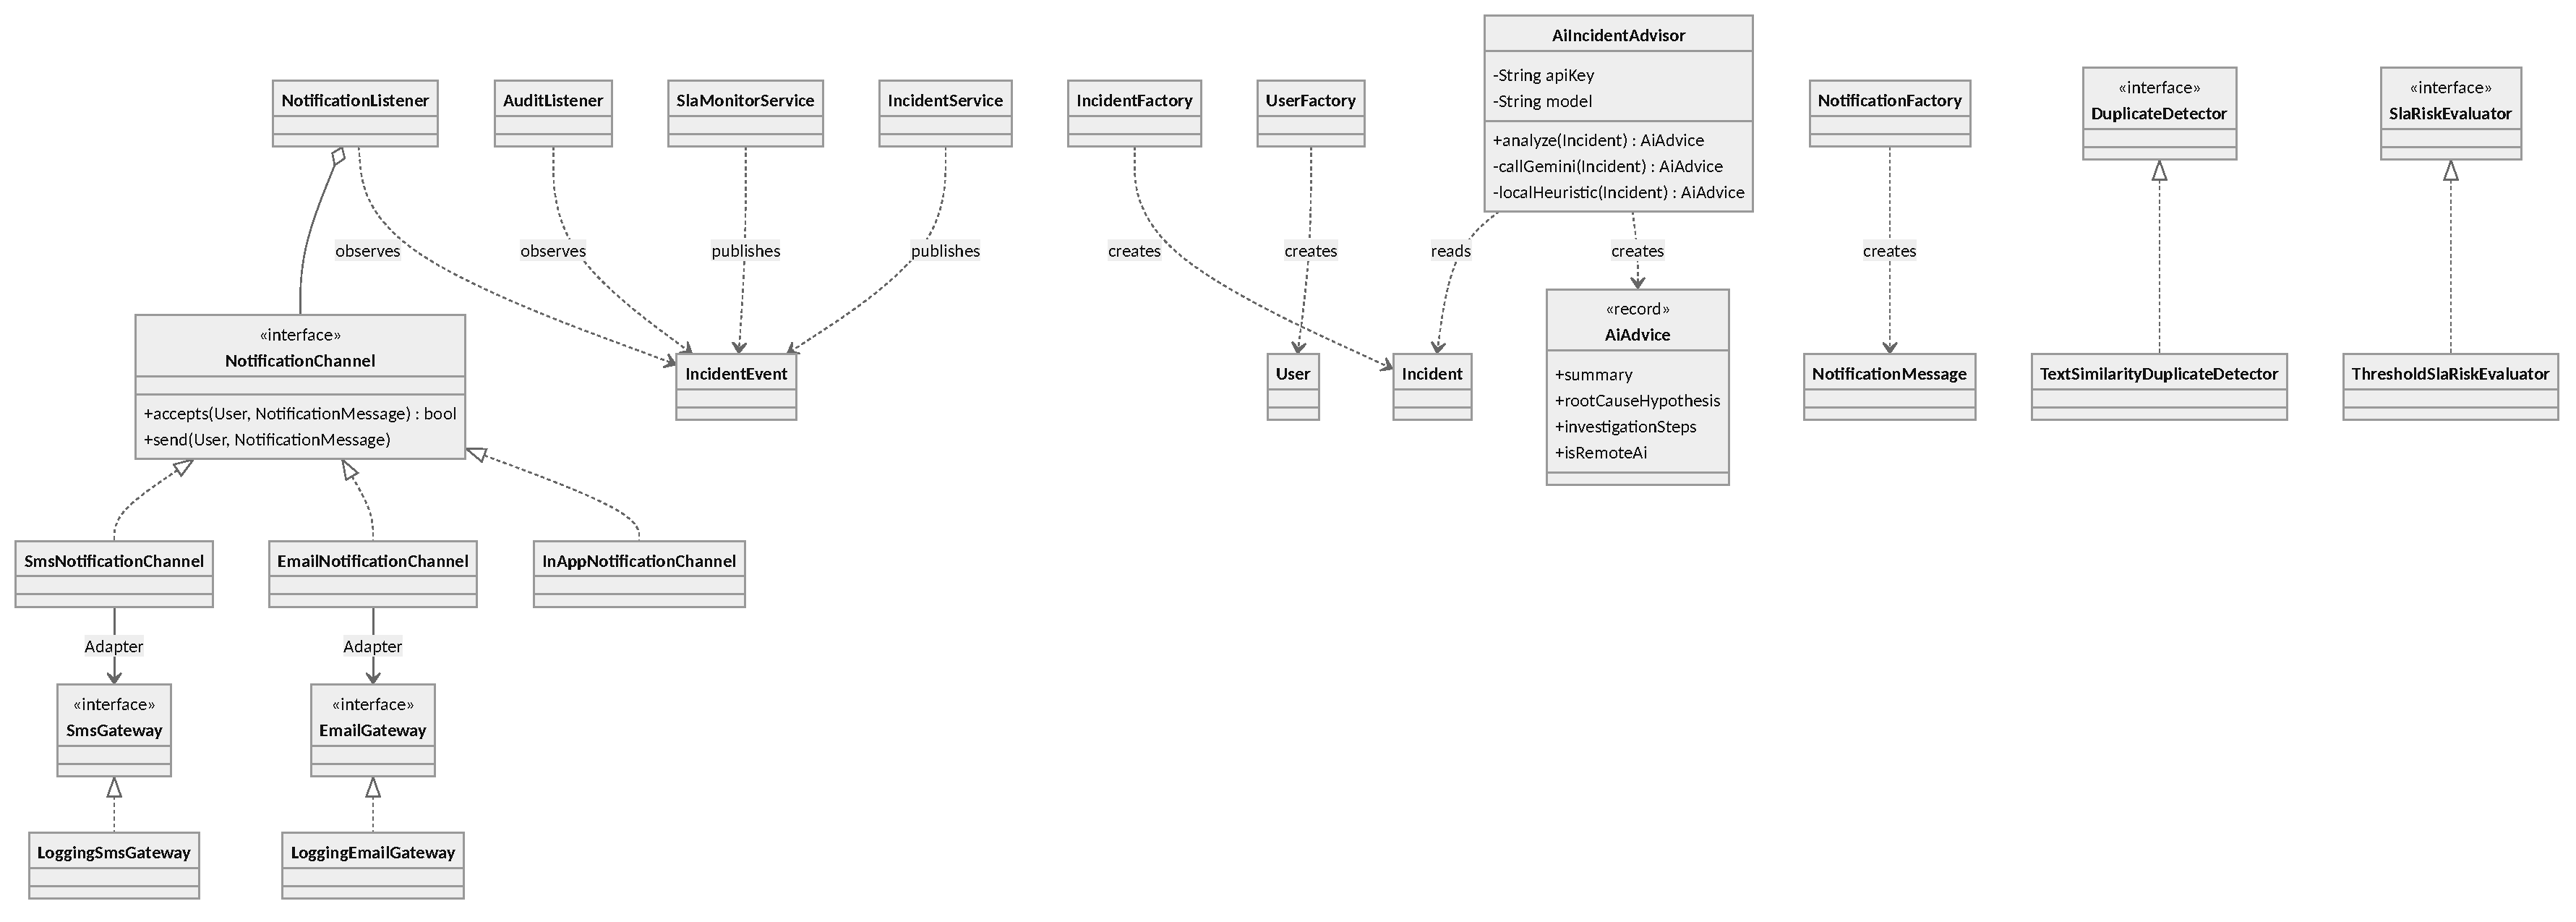
\includegraphics[width=\linewidth]{figures/pattern-observer.pdf}\caption{Observer (events $\rightarrow$ audit and notifications), Adapter (e-mail / SMS gateways), Factory, and the intelligence interfaces}\end{subfigure}
\caption{Design-pattern class diagrams}
\end{figure}

\subsubsection*{Where each pattern is used}
\begin{longtable}{@{}L{2.3cm}L{5.4cm}L{7.5cm}@{}}
\toprule
\textbf{Pattern} & \textbf{Where} & \textbf{Why} \\
\midrule\endhead
State & \code{IncidentState}, 9 state classes, \code{IncidentStateRegistry} & Each status allows only its own transitions; illegal ones are rejected in one place, with no \code{switch} on status. \\
Strategy & \code{PriorityStrategy} (2), \code{AssignmentStrategy} (4), \code{NotificationChannel} (3) & Algorithms are interchangeable: priority by configuration, assignment at runtime by an administrator. \\
Observer & \code{IncidentEvent} $\rightarrow$ \code{AuditListener}, \code{NotificationListener} & Services do not know who reacts; new reactions need no change to the services. \\
Factory & \code{IncidentFactory}, \code{UserFactory}, \code{NotificationFactory} & Creation rules (defaults, password hashing, message text) live in one place. \\
Repository & Spring Data interfaces, \code{IncidentSpecifications} & Persistence hidden behind interfaces; search filters compose. \\
Adapter & \code{EmailGateway} / \code{SmsGateway}; \code{ItsmUserPrincipal} & External providers and Spring Security plug in without touching domain logic. \\
\bottomrule
\end{longtable}

\subsection{State diagram}
\begin{figure}[H]\centering
\begin{minipage}[c]{0.42\linewidth}\centering
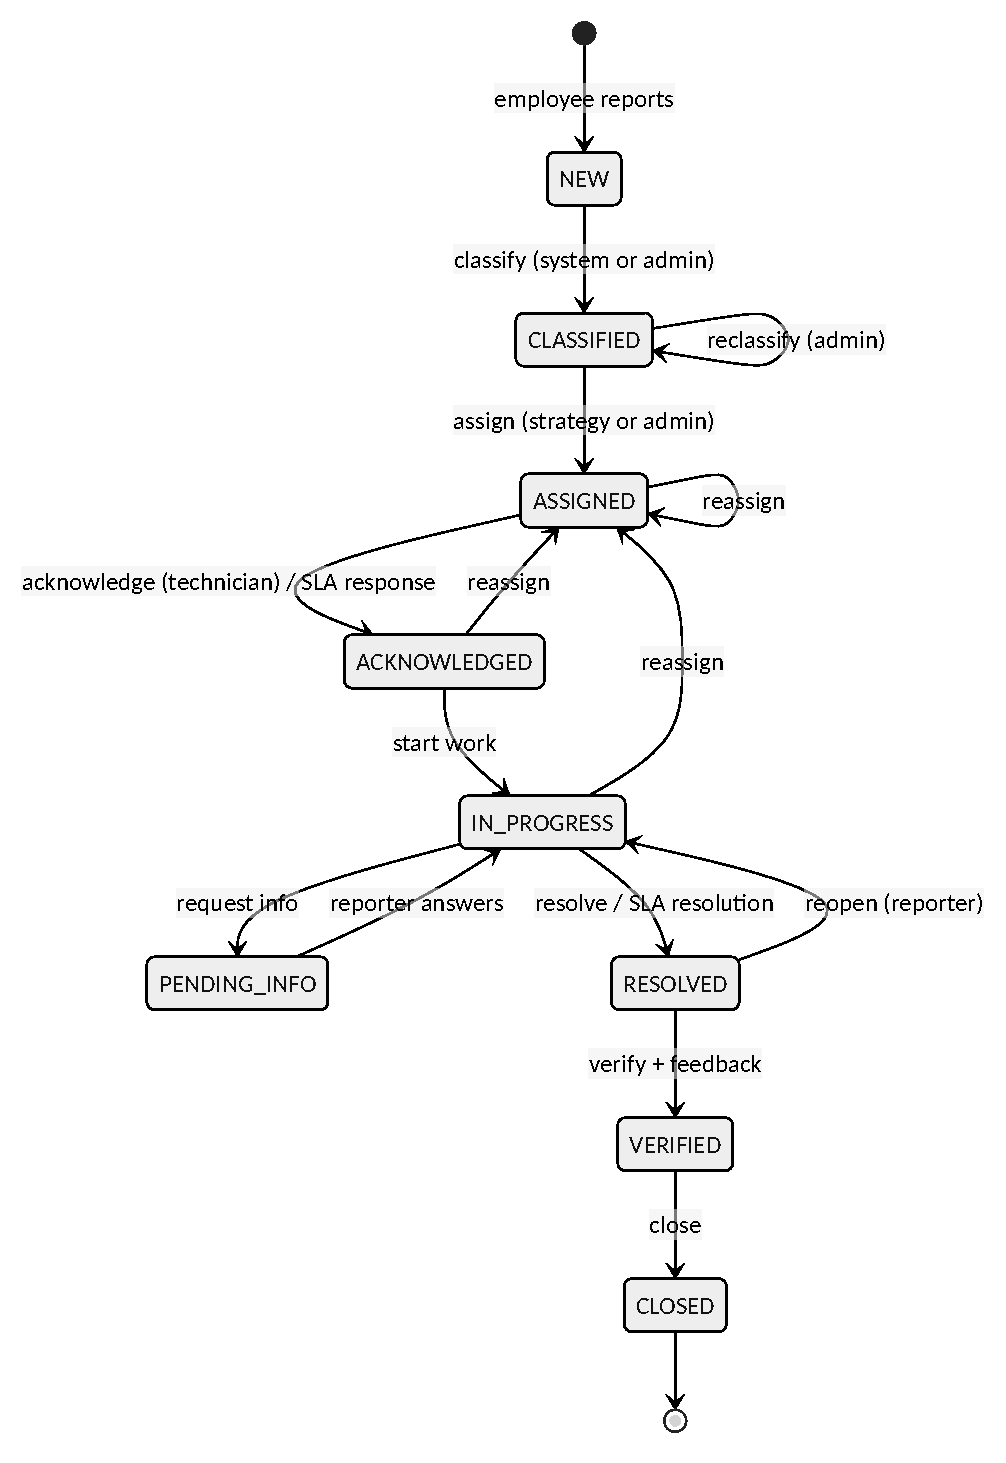
\includegraphics[width=\linewidth]{figures/state-machine.pdf}
\end{minipage}\hfill
\begin{minipage}[c]{0.54\linewidth}
\small The incident lifecycle follows the brief: NEW $\rightarrow$ CLASSIFIED $\rightarrow$ ASSIGNED $\rightarrow$ ACKNOWLEDGED $\rightarrow$ IN\_PROGRESS $\rightarrow$ RESOLVED $\rightarrow$ VERIFIED $\rightarrow$ CLOSED, plus PENDING\_INFO when the technician needs an answer and \textit{reopen} from RESOLVED.

Each status is a class implementing \code{IncidentState}. A state answers only the operations it allows and rejects the rest with \code{InvalidStateTransitionException}, so a jump such as NEW $\rightarrow$ CLOSED is impossible. \code{IncidentStateTest} checks all 90 (status, operation) pairs.
\end{minipage}
\caption{Incident lifecycle (State pattern)}
\end{figure}

\begin{landscape}
\subsection{Sequence diagram}
\begin{figure}[H]\centering
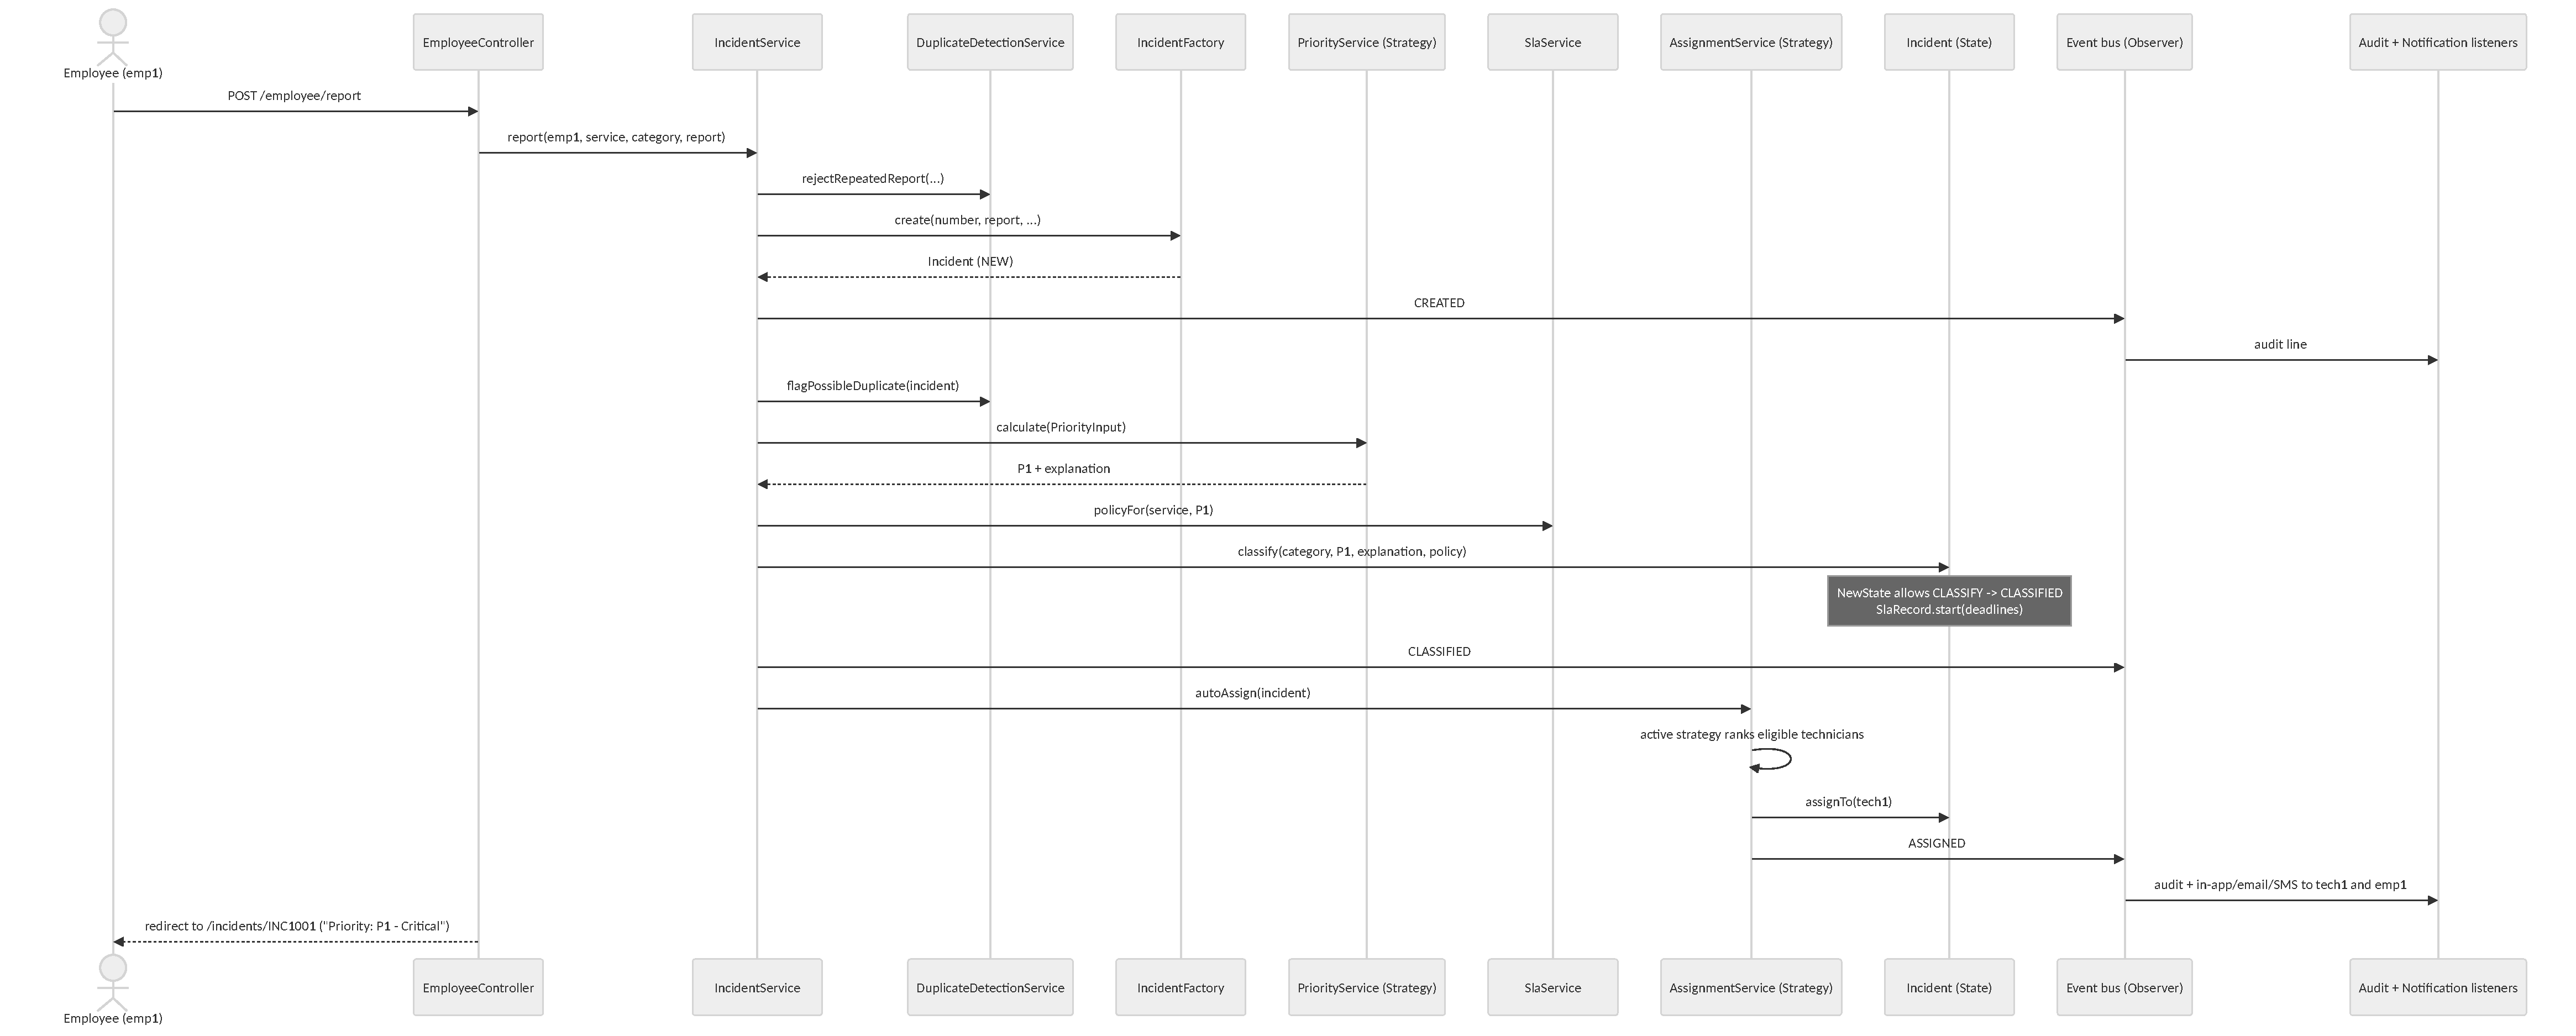
\includegraphics[height=0.82\textheight,width=\linewidth,keepaspectratio]{figures/sequence.pdf}
\caption{Sequence diagram for workflow 1: an employee reports, the system classifies and prioritises, assigns a technician and notifies through the event bus.}
\end{figure}
\end{landscape}

% ================================================================== Detailed design
\section{Detailed Design of the Main Modules}
This chapter explains how each major requirement of the brief is realised in code, with the rules, the algorithms and short excerpts from the source. Every excerpt is copied from the repository; import lines and some comments are left out, and long lines are re-wrapped to fit the page.

\subsection{Incident lifecycle (State pattern)}
The brief requires a well-defined lifecycle that prevents inappropriate transitions. The persisted status is a simple enum (\code{IncidentStatus}); \code{IncidentStateRegistry}, an \code{EnumMap}, maps every status to one stateless object implementing \code{IncidentState}. \code{AbstractIncidentState} rejects every operation by default, and each concrete state overrides only the operations it allows, so a new or forgotten operation is safe by construction.

\begin{longtable}{@{}L{2.9cm}L{4.4cm}L{7.9cm}@{}}
\toprule
\textbf{Status} & \textbf{Allowed operations} & \textbf{Result} \\
\midrule\endhead
NEW & classify & $\rightarrow$ CLASSIFIED (priority calculated, SLA clock started) \\
CLASSIFIED & classify, assign & re-classify (stays CLASSIFIED); assign $\rightarrow$ ASSIGNED \\
ASSIGNED & acknowledge, assign & acknowledge $\rightarrow$ ACKNOWLEDGED (response time recorded); reassign \\
ACKNOWLEDGED & start work, assign & start $\rightarrow$ IN\_PROGRESS; reassign $\rightarrow$ ASSIGNED \\
IN\_PROGRESS & request info, resolve, assign & request $\rightarrow$ PENDING\_INFO; resolve $\rightarrow$ RESOLVED (resolution time recorded) \\
PENDING\_INFO & provide info & reporter answers $\rightarrow$ IN\_PROGRESS \\
RESOLVED & verify, reopen & verify $\rightarrow$ VERIFIED; reopen $\rightarrow$ IN\_PROGRESS \\
VERIFIED & close & $\rightarrow$ CLOSED \\
CLOSED & none & final state; every operation is rejected \\
\bottomrule
\end{longtable}

\begin{lstlisting}[caption={The state contract and its default ``reject everything'' base class}]
public interface IncidentState {
    IncidentStatus status();
    Set<IncidentOperation> allowedOperations();      // drives which buttons the UI shows
    IncidentStatus classify();
    IncidentStatus assign();
    IncidentStatus acknowledge();
    // ... startWork, requestInfo, provideInfo, resolve, verify, reopen, close
}

abstract class AbstractIncidentState implements IncidentState {
    protected final IncidentStatus reject(IncidentOperation operation) {
        throw new InvalidStateTransitionException(status, operation);
    }
    @Override public IncidentStatus classify() { return reject(IncidentOperation.CLASSIFY); }
    @Override public IncidentStatus close()    { return reject(IncidentOperation.CLOSE); }
    // ... every other operation is rejected in the same way
}

final class AssignedState extends AbstractIncidentState {
    AssignedState() {
        super(IncidentStatus.ASSIGNED,
              EnumSet.of(IncidentOperation.ACKNOWLEDGE, IncidentOperation.ASSIGN));
    }
    @Override public IncidentStatus acknowledge() { return IncidentStatus.ACKNOWLEDGED; }
    @Override public IncidentStatus assign()      { return IncidentStatus.ASSIGNED; }
}
\end{lstlisting}

Responsibilities are split deliberately (decision D9): a \emph{state} decides whether an operation is legal and which status follows; the \code{Incident} asks its state first and only then changes its own fields, so a rejected operation leaves the object untouched; \code{IncidentService} decides \emph{who} may perform the operation (reporter, assignee or administrator) and publishes the resulting event.

\subsection{Priority determination (Strategy pattern)}
Priority is never typed in by a user. \code{PriorityService} delegates to the configured \code{PriorityStrategy}; two strategies are provided and the active one is chosen in \code{application.yml}.

\subsubsection*{Weighted scoring (default)}
\[ \textit{score} = \textit{impact}\,(1\text{--}3) \times \textit{urgency}\,(1\text{--}3) \times \textit{business criticality}\,(1\text{--}5) \times \textit{user factor} \]

\begin{tabularx}{\linewidth}{@{}YYYY@{}}
\toprule
\textbf{Affected users} & \textbf{User factor} & \textbf{Score} & \textbf{Priority} \\
\midrule
1--9 & 1.0 & $\geq 30$ & P1 Critical \\
10--99 & 1.2 & 15 -- 29.9 & P2 High \\
100--999 & 1.5 & 6 -- 14.9 & P3 Medium \\
1000 or more & 2.0 & below 6 & P4 Low \\
\bottomrule
\end{tabularx}

\begin{tabularx}{\linewidth}{@{}L{3.6cm}L{2.6cm}Y L{1.2cm}@{}}
\toprule
\textbf{Example} & \textbf{Inputs} & \textbf{Working} & \textbf{Result} \\
\midrule
Payment application down & High, High, crit.\ 5, 500 users & $3 \times 3 \times 5 = 45$; $\times 1.5 = 67.5$ & P1 \\
VPN split tunnelling broken & Medium, High, crit.\ 4, 40 users & $2 \times 3 \times 4 = 24$; $\times 1.2 = 28.8$ & P2 \\
E-mail delays & Medium, Medium, crit.\ 3, 5 users & $2 \times 2 \times 3 = 12$; $\times 1.0 = 12$ & P3 \\
HR portal cosmetic issue & Low, Low, crit.\ 2, 1 user & $1 \times 1 \times 2 = 2$; $\times 1.0 = 2$ & P4 \\
\bottomrule
\end{tabularx}

\begin{lstlisting}[caption={WeightedScoringPriorityStrategy.calculate}]
@Override
public PriorityResult calculate(PriorityInput input) {
    int base = input.impact().weight() * input.urgency().weight() * input.businessCriticality();
    double factor = affectedUsersFactor(input.affectedUsers());
    double score = base * factor;
    Priority priority = toPriority(score);
    String explanation = String.format(Locale.ROOT,
            "Impact %s(%d) x Urgency %s(%d) x Criticality %d = %d; "
                + "x %.1f for %d affected user(s) = %.1f -> %s",
            input.impact().label(), input.impact().weight(),
            input.urgency().label(), input.urgency().weight(),
            input.businessCriticality(), base, factor, input.affectedUsers(),
            score, priority.display());
    return new PriorityResult(priority, explanation);
}
\end{lstlisting}

The explanation string is stored on the incident and shown on its page, so the result is always auditable (Figure~\ref{fig:created}).

\subsubsection*{ITIL matrix (alternative)}
\code{MatrixPriorityStrategy} implements the classic impact $\times$ urgency matrix with a nested \code{EnumMap}. It ignores criticality and affected users, which is simpler but less precise; the test suite shows that the same input gives P1 with the weighted strategy and P3 with the matrix, which demonstrates polymorphism through one interface.

\begin{tabularx}{0.62\linewidth}{@{}l YYY@{}}
\toprule
 & \textbf{Urgency High} & \textbf{Medium} & \textbf{Low} \\
\midrule
\textbf{Impact High} & P1 & P2 & P3 \\
\textbf{Impact Medium} & P2 & P3 & P4 \\
\textbf{Impact Low} & P3 & P4 & P4 \\
\bottomrule
\end{tabularx}

\subsection{Technician assignment (Strategy pattern with a runtime registry)}
\code{AssignmentService} first filters eligible technicians (active, available and below their maximum workload) and then asks the active \code{AssignmentStrategy} to rank them. \code{AssignmentStrategyRegistry} receives every strategy from Spring as a list, and the administrator switches the active one on the \emph{Assignment strategy} screen; the choice is stored as a setting, so no code changes and no restart are needed.

\begin{longtable}{@{}L{3.3cm}L{7.6cm}L{4.3cm}@{}}
\toprule
\textbf{Strategy} & \textbf{Rule} & \textbf{Data structure} \\
\midrule\endhead
Skill-based (default) & Only technicians skilled in the incident's category; least busy first. & Stream filter + comparator \\
Load-based & Least busy technician first, regardless of skills. & \code{PriorityQueue} (min-heap) \\
Round-robin & Rotates among skilled technicians in turn, per category. & \code{ConcurrentHashMap} of \code{AtomicInteger} \\
Smart recommendation (feature D) & Score out of 100 with an explanation (below). & Sorted list of scores \\
\bottomrule
\end{longtable}

\begin{lstlisting}[caption={The assignment contract and the load-based strategy}]
public interface AssignmentStrategy {
    String name();
    String description();
    List<TechnicianScore> rank(Incident incident, List<Candidate> candidates);
    default Optional<Technician> select(Incident incident, List<Candidate> candidates) {
        return rank(incident, candidates).stream().findFirst().map(TechnicianScore::technician);
    }
}

@Component
public class LoadBasedAssignmentStrategy implements AssignmentStrategy {
    @Override
    public List<TechnicianScore> rank(Incident incident, List<Candidate> candidates) {
        PriorityQueue<Candidate> byLoad = new PriorityQueue<>(
                Comparator.comparingInt(Candidate::activeIncidents)
                          .thenComparing(Candidate::username));
        byLoad.addAll(candidates);
        List<TechnicianScore> ranking = new ArrayList<>(candidates.size());
        while (!byLoad.isEmpty()) {
            Candidate c = byLoad.poll();
            ranking.add(new TechnicianScore(c.technician(), 100 - c.activeIncidents(),
                    c.activeIncidents(), c.activeIncidents() + " active incident(s) of max "
                    + c.technician().getMaxWorkload()));
        }
        return ranking;
    }
}
\end{lstlisting}

\subsubsection*{Smart recommendation score}
\[ 40 \cdot \textit{skill} + 25 \cdot (1 - \tfrac{\textit{active}}{\textit{max}}) + 15 \cdot \tfrac{\textit{experience}}{5} + 10 \cdot \tfrac{\min(\textit{handled on service},\,5)}{5} + 10 \cdot [\textit{P1/P2 and senior}] \]
Worked example: a P1 database incident and a database-skilled technician with 1 of 5 incidents active, experience level 5 and 3 past incidents on the service scores $40 + 20 + 15 + 6 + 10 = 91$. A technician without the skill, otherwise identical, scores 51. The administrator sees the score and its breakdown in the assignment drop-down (``Why these scores?'').

\subsection{SLA management}
\code{SlaService} finds the applicable \code{SlaPolicy}: a policy for the incident's service and priority if one exists, otherwise the default policy for the priority; if neither exists, \code{MissingSlaConfigurationException} is raised. The deadlines are stored in the embedded \code{SlaRecord}, and the incident records the response time when it is acknowledged and the resolution time when it is resolved, so no caller can forget to do it.

\begin{tabularx}{\linewidth}{@{}L{2cm}L{3.2cm}L{3.4cm}Y@{}}
\toprule
\textbf{Priority} & \textbf{Response target} & \textbf{Resolution target} & \textbf{Demo override} \\
\midrule
P1 & 5 minutes & 30 minutes & Payment Gateway: 2 min / 10 min \\
P2 & 15 minutes & 2 hours & -- \\
P3 & 1 hour & 8 hours & -- \\
P4 & 4 hours & 24 hours & -- \\
\bottomrule
\end{tabularx}

The background \code{SlaMonitor} (\code{@Scheduled}, every 20 seconds) asks \code{SlaMonitorService} to check every open incident. A deadline that passes marks the record BREACHED once and permanently and publishes \code{SLA\_VIOLATED}; an incident that the \code{SlaRiskEvaluator} judges to be at risk publishes \code{SLA\_APPROACHING} once (feature E).

\begin{lstlisting}[caption={ThresholdSlaRiskEvaluator: when is an incident at risk?}]
@Override
public boolean isAtRisk(Incident incident, Instant now, long assigneeActiveIncidents) {
    SlaRecord sla = incident.getSlaRecord();
    if (!sla.isStarted() || sla.getStatus() != SlaStatus.ON_TRACK
            || !incident.getStatus().isOpen()) {
        return false;
    }
    // 75% of the response window has passed and nobody has acknowledged it
    if (sla.getRespondedAt() == null
            && fraction(incident.getCreatedAt(), sla.getResponseDue(), now) >= threshold) {
        return true;
    }
    double resolution = sla.elapsedFraction(incident.getCreatedAt(), now);
    if (resolution >= threshold) {
        return true;                                   // 75% of the resolution window
    }
    // 50% of the window has passed and the assigned technician is at least 80% busy
    Technician tech = incident.getAssignee();
    return tech != null && resolution >= BUSY_ELAPSED
            && assigneeActiveIncidents >= BUSY_LOAD * tech.getMaxWorkload();
}
\end{lstlisting}

\subsection{Events, audit trail and notifications (Observer, Strategy, Adapter, Factory)}
Every state change publishes an immutable \code{IncidentEvent} (type, incident number, actor, previous and new status, description, time). Services never call audit or notification code directly. Two observers listen, synchronously and inside the same transaction:
\begin{itemize}
  \item \code{AuditListener} writes one \code{AuditEntry} per event, so an incident change and its audit line are saved together or not at all;
  \item \code{NotificationListener} looks up the recipients in a rule table (an \code{EnumMap}) and sends the message through every channel that accepts it. A failing channel is logged and skipped; it never blocks the update.
\end{itemize}

\begin{longtable}{@{}L{4.4cm}L{5.4cm}L{5.4cm}@{}}
\toprule
\textbf{Event} & \textbf{Who is notified} & \textbf{Channels} \\
\midrule\endhead
Created, classified & Reporter & In-app, e-mail \\
Technician assigned & Reporter, assigned technician & In-app, e-mail; SMS to the technician if P1/P2 \\
No technician available & All administrators & In-app, e-mail, SMS \\
Acknowledged, work started & Reporter & In-app, e-mail \\
Information requested / provided & Reporter / technician & In-app, e-mail \\
Resolved, closed & Reporter (and technician on close) & In-app, e-mail \\
Verified, reopened & Assigned technician & In-app, e-mail \\
SLA approaching & Technician, team leads & In-app, e-mail, SMS \\
SLA violated & Technician, team leads, administrators & In-app, e-mail, SMS \\
Escalated & Technician, escalation target & In-app, e-mail, SMS \\
Duplicate detected / confirmed & Technician / reporter & In-app, e-mail \\
\bottomrule
\end{longtable}

\begin{lstlisting}[caption={The audit observer and the SMS channel, which uses the SmsGateway adapter}]
@Component
public class AuditListener {
    @EventListener
    @Order(0) // record the audit line before notifications are attempted
    public void on(IncidentEvent event) {
        String description = event.description() == null
                ? event.type().label() : event.type().label() + ": " + event.description();
        auditEntries.save(new AuditEntry(event.occurredAt(), event.actor(), event.type().name(),
                event.incidentNumber(), event.previousStatus(), event.newStatus(),
                truncate(description)));
    }
}

@Component
public class SmsNotificationChannel implements NotificationChannel {
    @Override public ChannelType type() { return ChannelType.SMS; }
    @Override public boolean accepts(User recipient, NotificationMessage message) {
        return message.urgent() && recipient.getPhone() != null;   // SMS only for urgent events
    }
    @Override public void send(User recipient, NotificationMessage message) {
        gateway.send(recipient.getPhone(), message.shortText());    // SmsGateway: Adapter target
        notifications.save(new Notification(recipient, ChannelType.SMS, message.subject(),
                message.shortText(), message.incidentNumber(), Instant.now(clock)));
    }
}
\end{lstlisting}

Channels per role come from configuration: employees receive in-app and e-mail messages only, while technicians and administrators also receive SMS for urgent events (SLA approaching or violated, escalation, no technician available, or a P1/P2 assignment). \code{NotificationFactory} builds the subject and text of every message in one place. The \code{EmailGateway} and \code{SmsGateway} interfaces are the Adapter targets: the demo uses \code{LoggingEmailGateway} and \code{LoggingSmsGateway}, which write to an outbox that administrators can inspect, and a real provider (SMTP, Twilio) would be one new class. Adding a push-notification channel would likewise be one new \code{NotificationChannel} implementation.

\shot{15-outbox}{The simulated e-mail and SMS outbox: every message produced by the notification channels.}

\subsection{Exception hierarchy}
\begin{figure}[H]
\centering
\begin{minipage}{0.92\linewidth}
\begin{lstlisting}[language={},numbers=none,caption={Custom exceptions (all unchecked)}]
RuntimeException
 +-- ItsmException (abstract)
      +-- NotFoundException (abstract)           -> 404 page
      |    +-- IncidentNotFoundException, ServiceNotFoundException,
      |        CategoryNotFoundException, UserNotFoundException
      +-- AssignmentException (abstract)
      |    +-- TechnicianUnavailableException, WorkloadExceededException
      +-- UnauthorizedOperationException          -> 403 page
      +-- InvalidStateTransitionException
      +-- InvalidInputException
      +-- MissingSlaConfigurationException
      +-- DuplicateIncidentException
      +-- ExternalServiceException                (gateways, AI API)
\end{lstlisting}
\end{minipage}
\end{figure}
\code{GlobalExceptionHandler} (\code{@ControllerAdvice}) handles each family once: not-found errors show the 404 page, unauthorised operations the 403 page, and the remaining domain errors return the user to the page they came from with a readable message. Because the hierarchy is shallow and grouped, a new exception is handled automatically by its parent's handler.

\subsection{Search and reporting}
The brief asks for at least five criteria; the search page offers ten, which can be combined freely. Each criterion is a small \code{Specification<Incident>} in \code{IncidentSpecifications} that returns nothing when its field is empty, so only the filters in use are combined. A visibility rule is always added: employees see only their own incidents and technicians the incidents they work on, while team leads and administrators see all.

\begin{tabularx}{\linewidth}{@{}L{3.4cm}Y@{}}
\toprule
\textbf{Criterion} & \textbf{Meaning} \\
\midrule
Incident number & Exact number, e.g. INC1001 \\
Text & Words in the title or description \\
From / to date & Reporting date range \\
Status, priority & Lifecycle status; P1--P4 \\
Category, service & Classification and affected IT service \\
Technician & Assigned technician \\
SLA status & Not started, on track, at risk, breached, met \\
\bottomrule
\end{tabularx}

\code{ReportService} builds the administrator overview: totals, open, open P1, resolved, SLA violations, compliance percentage and average resolution time, the at-risk list, unassigned incidents, technician workload, outage hotspots (feature B) and breakdowns by service, category, priority and status, which also feed the charts. Search results and the audit log can be exported as CSV.

\subsection{Users and factories}
\code{User} is abstract; \code{Employee}, \code{Technician} and \code{Administrator} add only what is specific to them (department; skills, workload, experience, availability and team-lead flag; IT-manager flag). \code{UserFactory} is the single place where users are created: it validates the details, hashes the password with BCrypt and returns the right subtype. \code{IncidentFactory} likewise turns an employee's \code{IncidentReport} into a valid NEW incident, applying defaults (medium impact and urgency, one affected user), length limits and a title derived from the description when none is given.


% ================================================================== 5
\section{Technology Stack}
\begin{tabularx}{\linewidth}{@{}L{3.2cm}Y@{}}
\toprule
\textbf{Layer} & \textbf{Technology} \\
\midrule
Language & Java 21 \\
Framework & Spring Boot 3.5: Web MVC, Security, Data JPA, Validation, Scheduling \\
User interface & Thymeleaf server-side templates; Bootstrap 5.3 and Bootstrap Icons (bundled as WebJars); Chart.js 4.4; light and dark themes \\
Persistence & Hibernate / JPA; PostgreSQL 16 (Docker Compose) for the demo; H2 in memory for tests and development \\
External API & Google Gemini \code{generateContent} REST API (optional, used when a key is configured) \\
Testing & JUnit 5, AssertJ, Mockito, Spring Boot Test, MockMvc, Spring Security Test \\
Build and tools & Maven, Git and GitHub, IntelliJ IDEA / VS Code \\
\bottomrule
\end{tabularx}

\subsection{Technology selection}
\begin{enumerate}[leftmargin=1.4em]
  \item \textbf{Why Java?} It is strongly object-oriented: interfaces, abstract classes, enums with behaviour, records for value objects. Every OOP requirement of the brief maps onto a language feature.
  \item \textbf{Why Thymeleaf and Bootstrap?} Pages are rendered on the server with Spring Security integration, so each role gets a different interface without a separate front-end project. Bootstrap gives a responsive layout, and its colour modes made the dark theme a matter of colour tokens.
  \item \textbf{Why Spring Boot?} Dependency injection makes the patterns natural: Spring injects every \code{AssignmentStrategy} into a registry, \code{ApplicationEvent\-Publisher} is a ready Observer bus, Spring Data generates repositories, and \code{@Scheduled} runs the SLA monitor.
  \item \textbf{Why PostgreSQL?} The data is strongly relational (users, incidents, services, SLA policies, audit) with integrity constraints and transactions. H2 keeps the tests fast; JPA runs the same code on both.
  \item \textbf{Why this architecture?} A layered application is the simplest structure that separates concerns, and it is easy to test, deploy and explain.
  \item \textbf{Alternatives considered:} React with a REST API (richer UI, but two code bases); Node.js or Django (less natural for an OOP-in-Java course); MongoDB (weaker fit for relational data); microservices (unnecessary operational cost at this scale).
  \item \textbf{Advantages and limitations.} Advantages: strong typing, framework support for the patterns, security out of the box, very testable. Limitations: pages need a reload to update (no live push), dashboard figures are aggregated in memory, and e-mail and SMS are simulated.
  \item \textbf{Support for OOP.} JPA maps the user inheritance hierarchy and the composition (\code{@Embedded}, cascades); Spring wires interfaces to implementations, so classes depend on abstractions; Bean Validation keeps input rules declarative.
  \item \textbf{Growth to many more users.} Run several stateless instances behind a load balancer with shared sessions; add indexes and move dashboard figures into SQL queries or a read replica; send notifications through a message queue; run the SLA monitor on one node with a lock; split notifications and reporting into services along the existing event boundaries.
\end{enumerate}

% ================================================================== 6
\needspace{10\baselineskip}
\section{Intelligent Features}\label{sec:intelligent}
The brief asks for at least two intelligent or automated features. I-ITSM implements all seven suggested (A--G) and three innovation extensions.

\begin{longtable}{@{}L{0.5cm}L{3.1cm}L{8.2cm}L{3.3cm}@{}}
\toprule
& \textbf{Feature} & \textbf{How it works} & \textbf{Class} \\
\midrule\endhead
A & Duplicate detection & Text is normalised (stop words, plurals, synonyms such as \textit{checkout / pay $\rightarrow$ payment}), then compared by Jaccard word overlap, +0.2 for the same service; flagged at 0.5. A person confirms or dismisses. & \code{TextSimilarity\-DuplicateDetector} \\
B & Incident correlation & Open incidents on the same service in the last 24 h are shown together; a ``possible outage'' banner appears when a service has two or more open reports in an hour. & \code{ReportService} \\
C & Automatic escalation & An unacknowledged P1/P2 escalates to the team lead, then the system administrator, then the IT manager; levels with nobody available are skipped. & \code{Escalation\-Service} \\
D & Smart recommendation & Score out of 100: skill 40, spare capacity 25, experience 15, history with the service 10, senior bonus 10 for P1/P2, with an explanation. & \code{Smart\-Recommendation\-Strategy} \\
E & SLA risk detection & At risk at 75\% of the window (50\% when the technician is at least 80\% busy); warned once. & \code{ThresholdSlaRisk\-Evaluator} \\
F & Category suggestion & Category keywords are matched against the description while the employee types. & \code{Category\-Suggester} \\
G & Suggested resolutions & Up to three similar resolved incidents, with their fix and root cause, are shown to the technician. & \code{Resolution\-Suggester} \\
+ & AI root-cause advisor & Calls the Google Gemini API when a key is set; otherwise uses local expert rules, so it always works offline. & \code{AiIncidentAdvisor} \\
+ & Service dependency graph & Services depend on other services; an incident shows the upstream services and the downstream services it may affect. & \code{ITService}, \code{CatalogService} \\
+ & Analytics and export & Chart.js dashboard; search results and audit log export to CSV. & \code{ReportService} \\
\bottomrule
\end{longtable}

Priority calculation is automated and explains itself, for example: \textit{Impact High(3) $\times$ Urgency High(3) $\times$ Criticality 5 = 45; $\times$ 1.5 for 500 affected users = 67.5 $\rightarrow$ P1 Critical.}

\subsection{Duplicate detection: a worked example}
\code{TextNormalizer} lower-cases the text, removes stop words and simple plurals, and maps synonyms onto one word: \textit{transaction, checkout, pay} $\rightarrow$ \textit{payment}; \textit{down, failing, unable, unavailable} $\rightarrow$ \textit{outage}. For the brief's example:

\begin{tabularx}{\linewidth}{@{}L{5.4cm}Y@{}}
\toprule
\textbf{Report} & \textbf{Normalised word set} \\
\midrule
``Payment application unavailable'' & \{payment, application, outage\} \\
``Payment transaction failing'' & \{payment, outage\} \\
\bottomrule
\end{tabularx}

Jaccard similarity $= |A \cap B| \,/\, |A \cup B| = 2/3 = 0.67$, plus 0.2 because both are on the Payment Gateway service, giving 0.87, above the threshold of 0.5. The new incident is linked to the \emph{original} report (never to another duplicate), and the technician confirms or dismisses the match. The same employee filing the same report again within an hour is refused outright with \code{DuplicateIncidentException}.

\subsection{Automatic escalation}
\code{EscalationService} watches P1 and P2 incidents that nobody has acknowledged yet (still CLASSIFIED or ASSIGNED). When the response deadline passes, the incident escalates to a team lead; one response window later to the system administrator; one more window later to the IT manager. A level with nobody available is skipped, each escalation is stored as an \code{Escalation} record and announced through the normal event flow (SMS included), and acknowledging the incident stops the chain. With the demo override for Payment Gateway P1 (two-minute response), the whole chain can be shown in a few minutes.

\subsection{AI incident advisor and service dependency graph}
\code{AiIncidentAdvisor} builds a short prompt from the incident (title, description, service, criticality, priority, affected users) and calls the Google Gemini \code{generateContent} REST endpoint through Java's \code{HttpClient} with short time-outs. If no key is configured, or the call fails, it falls back to local expert rules per service type, so the incident page always shows a triage summary, a root-cause hypothesis and investigation steps. Each \code{ITService} holds a set of services it depends on (a self-referencing many-to-many association); the incident page shows the upstream services and the downstream services that may also be affected, for example an Auth / SSO outage warns about Payment Gateway, VPN, E-mail and HR Portal.

\twoshots{05-duplicate-flagged}{A second report of the payment outage is flagged as a possible duplicate of INC1001 (similarity 0.60).}{07-tech-incident}{The technician's view: suggested resolutions from similar past incidents, AI advisor and dependency impact.}

% ================================================================== 7
\section{Database Design}
The schema has 12 tables and is generated by Hibernate from the entities (\code{create-drop} on H2, \code{update} on PostgreSQL).

\begin{landscape}
\begin{figure}[H]\centering
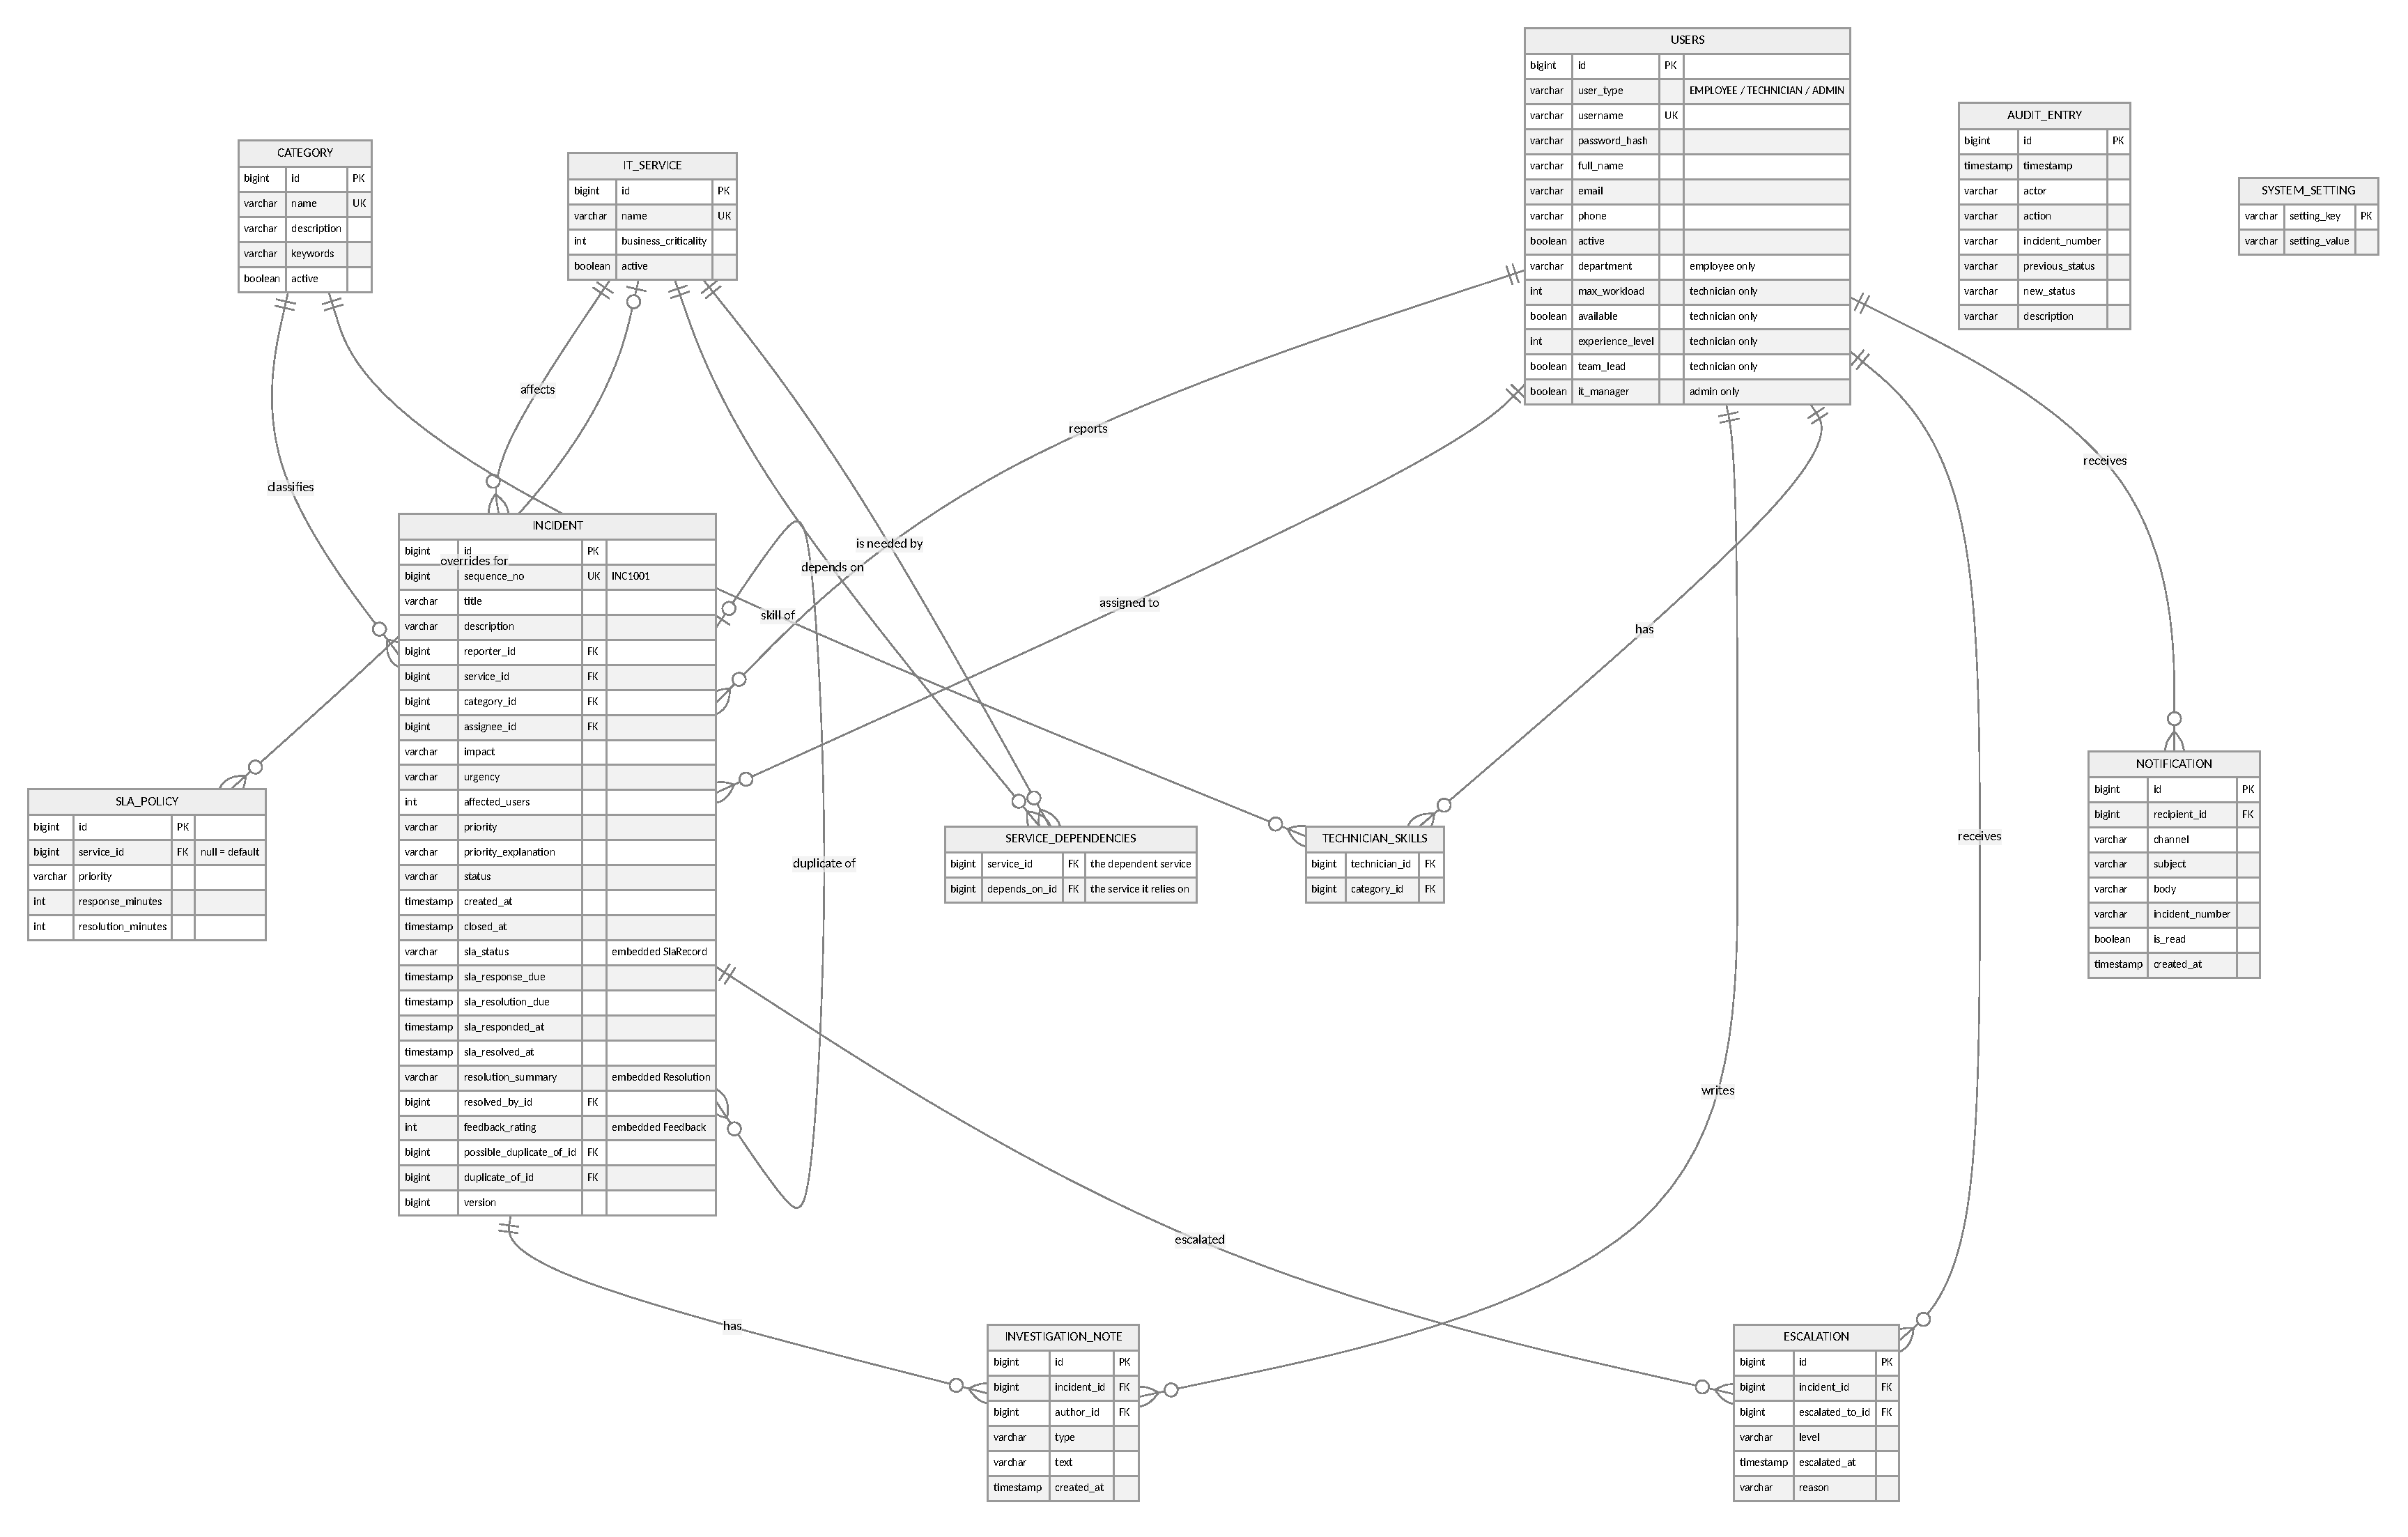
\includegraphics[height=0.84\textheight,width=\linewidth,keepaspectratio]{figures/er.pdf}
\caption{Entity--relationship diagram}
\end{figure}
\end{landscape}

\subsection{Tables}
\begin{longtable}{@{}L{4cm}L{11.2cm}@{}}
\toprule
\textbf{Table} & \textbf{Purpose and key columns} \\
\midrule\endhead
\code{users} & All users (single-table inheritance): username, BCrypt password hash, name, contact details, active flag, \code{user\_type}; employee department; technician capacity, availability, experience, team-lead flag; administrator IT-manager flag. \\
\code{incident} & The incident aggregate: sequence number (shown as INC1001), title, description, reporter, service, category, assignee, impact, urgency, affected users, priority and its explanation, status, timestamps; embedded SLA record, resolution and feedback; duplicate links; \code{version}. \\
\code{investigation\_note} & Notes, questions and answers on an incident, with author, type and time. \\
\code{it\_service} & IT services with business criticality (1--5) and an active flag. \\
\code{service\_dependencies} & Service-to-service dependencies (self-join) for impact analysis. \\
\code{category} & Incident categories with keywords for suggestion; data, not an enum. \\
\code{technician\_skills} & Many-to-many link between technicians and categories. \\
\code{sla\_policy} & Response and resolution minutes per priority, optionally per service. \\
\code{escalation} & Escalation history: incident, level, target user, time and reason. \\
\code{audit\_entry} & Audit trail: time, actor, action, incident number, previous and new status, description. \\
\code{notification} & Delivered notifications: recipient, channel, subject, body, incident, read flag. \\
\code{system\_setting} & Key--value settings, such as the active assignment strategy. \\
\bottomrule
\end{longtable}

\subsection{Important relationships}
\begin{itemize}
  \item An incident has one reporter, one affected service, at most one category and at most one assigned technician.
  \item An incident owns many investigation notes and escalations; an incident may point to another as its duplicate.
  \item Technicians and categories are many-to-many (\code{technician\_skills}); services depend on services (\code{service\_dependencies}).
  \item An SLA policy belongs to a service, or to no service for the default policy.
\end{itemize}

\subsection{Design choices}
\begin{itemize}
  \item Single-table inheritance for the user hierarchy: one \code{users} table with a type column.
  \item SLA record, resolution and feedback are embedded in the incident row (composition).
  \item The audit trail stores the incident number as text, so history is never lost; a \code{version} column provides optimistic locking.
\end{itemize}

\subsection{Sample data}
On an empty database the application creates 9 demo accounts (3 employees, 3 technicians, 1 team lead, 2 administrators), 7 services with dependencies (for example, Payment Gateway depends on Core Database and Auth / SSO), 9 categories, default SLA policies plus a fast Payment Gateway override for the demo, and 28 historical incidents with resolutions, feedback, breaches and audit history.

% ================================================================== 8
\section{Security and Exception Handling}\label{sec:security}
\begin{tabularx}{\linewidth}{@{}L{3.6cm}Y@{}}
\toprule
\textbf{Requirement} & \textbf{Implementation} \\
\midrule
Authentication & Spring Security form login; invalid login returns to the login page; disabled accounts cannot log in. \\
Role-based authorisation & URL rules for \code{/employee}, \code{/tech}, \code{/admin}; \code{@PreAuthorize} on administration services; ownership checks in \code{IncidentService}. Three independent layers. \\
Password protection & BCrypt (salted, deliberately slow); passwords are never logged. \\
Input validation & Bean Validation on every form; domain constructors validate again. \\
Secure access & Every page and the JSON endpoint require login; CSRF token on every form; output escaped by Thymeleaf; bound SQL parameters. \\
Unauthorised operations & \code{UnauthorizedOperationException} returns a 403 page; the interface shows only permitted actions. \\
\bottomrule
\end{tabularx}

Not implemented, and stated: two-factor authentication, login rate limiting, HTTPS termination (a reverse proxy would provide it) and password reset by e-mail.

\subsection{Exception handling}
All custom exceptions extend \code{ItsmException} and are handled by a single \code{GlobalExceptionHandler}, which turns each family into a friendly message or error page.

\begin{tabularx}{\linewidth}{@{}L{5.2cm}Y@{}}
\toprule
\textbf{Situation from the brief} & \textbf{Exception / handling} \\
\midrule
Invalid login & Spring Security failure handler, message on the login page \\
Unauthorised operation & \code{UnauthorizedOperationException} (403 page) \\
Invalid incident / service not found & \code{IncidentNotFoundException}, \code{ServiceNotFoundException} (404 page) \\
Invalid state transition & \code{InvalidStateTransitionException} \\
Technician unavailable / workload exceeded & \code{TechnicianUnavailableException}, \code{WorkloadExceededException} \\
Missing SLA configuration & \code{MissingSlaConfigurationException} \\
Duplicate incident & \code{DuplicateIncidentException} \\
Database / network failure & Spring \code{DataAccessException} handler; \code{ExternalServiceException} for gateways and the AI API \\
Invalid user input & \code{InvalidInputException} and form validation errors \\
\bottomrule
\end{tabularx}

% ================================================================== 9
\section{Testing}
The project has \textbf{249 automated tests in 27 test classes}, all passing with \code{mvn test}, and \textbf{108 documented test cases} (Appendix~\ref{app:tests}). Techniques: plain unit tests for the domain and strategies; \code{@DataJpaTest} with a real H2 database for repositories and services; a \code{MutableClock} to move time forward; \code{@SpringBootTest} with MockMvc and Spring Security Test for the web layer; recorded application events to verify the Observer flow. A selection:

\begin{longtable}{@{}L{1.1cm}L{2.2cm}L{5.8cm}L{6cm}@{}}
\toprule
\textbf{ID} & \textbf{Type} & \textbf{Scenario} & \textbf{Expected result} \\
\midrule\endhead
TC22 & Normal & Report $\rightarrow$ classify $\rightarrow$ assign $\rightarrow$ acknowledge $\rightarrow$ start $\rightarrow$ request/provide info $\rightarrow$ resolve $\rightarrow$ verify $\rightarrow$ close & Ends CLOSED with resolution, feedback and notes \\
TC34 & Business rule & Brief's examples: payment outage, VPN, e-mail, HR portal & P1, P2, P3, P4 \\
TC49 & Normal & Skill-based assignment with two database technicians and one network technician & Only database technicians; least busy first \\
TC52 & Normal & Round-robin over three incidents & Turns rotate among skilled technicians \\
TC19 & Normal & Service-specific versus default SLA policy & Specific policy for that service, default otherwise \\
TC94 & Normal & Search by category and status together & Both filters applied (AND) \\
TC13 & Boundary & Technician at 2/3 versus 3/3 workload & Has capacity at 2, not at 3 \\
TC40 & Boundary & Response exactly at the 5-minute deadline & Not a breach \\
TC88 & Boundary & P1 at 73\%, 77\%, 80\% of its window, then past the deadline & Warning at 77\% only, once; breach reported once \\
TC106 & Boundary & AI advisor on a NEW incident that has no priority yet & Advice produced; page renders (regression test) \\
TC07 & Invalid input & Blank or ``bad name!'' username & \code{InvalidInputException} \\
TC10 & Invalid input & Blank title, no service, 0 affected users & \code{InvalidInputException} \\
TC76 & Invalid input & Report form submitted empty & Form shown again with field errors \\
TC23 & Exception & Illegal operation on a NEW incident & Exception thrown, no field changed \\
TC31 & Exception & Assign to an unavailable technician & \code{TechnicianUnavailableException} \\
TC85 & Exception & Same employee repeats a report within one hour & \code{DuplicateIncidentException} naming the original \\
TC67 & Exception & No technician available for a P1 & Administrators alerted (in-app and SMS) \\
TC70 & Authorisation & Anonymous user opens \code{/employee} & Redirected to login \\
TC73 & Authorisation & Employee opens \code{/admin}; technician opens the report form & 403 \\
TC79 & Authorisation & Technician resolves another's incident; employee views another's incident & 403 \\
TC28 & Authorisation & Employee tries to resolve & \code{UnauthorizedOperationException} \\
TC43 & Business rule & Deadline passes and is checked repeatedly & Breach reported only once \\
TC91 & Business rule & Technician acknowledges after the first escalation & No further escalations \\
TC105 & Normal & Export search results to CSV & 200, \code{text/csv}, attachment \\
\bottomrule
\end{longtable}

Manual testing covered every page as each role and the three demonstration workflows. Three defects found this way were fixed with regression tests: escalation stalling when the only team lead was the assignee, the start-up order of default SLA policies, and an error page for brand-new incidents caused by the AI advisor (TC106).

% ================================================================== 10
\section{Project Demonstration}
The recorded video (\videoname, 15--20 minutes) demonstrates three complete workflows; every member introduces themselves and explains their module. The screenshots below were taken from the running application.

\subsection{Workflow 1: report, prioritise, assign, notify}
\twoshots{01-login}{Login page with the light / dark theme switch.}{03-report-form}{The employee reports the payment outage; a category is suggested from the text (feature F).}

\shot{04-incident-created}{\label{fig:created}The incident is created, classified and prioritised P1 with the working shown, auto-assigned to Karan Shah by the skill strategy, and its SLA clock started.}

\twoshots{06-tech-queue}{The technician's queue, most urgent SLA first, with current workload.}{08-notifications}{The technician is notified of the assignment (in-app; e-mail and SMS go to the outbox).}

\subsection{Workflow 2: investigate, monitor SLA, resolve, notify}
The technician acknowledges the incident (response time recorded against the SLA), starts the investigation, adds notes and can ask the reporter a question, which moves the incident to PENDING\_INFO until the reporter answers. The SLA countdown and risk badges stay visible throughout.

\twoshots{22-tech-queue-pending}{A team lead's queue: the incident waiting for the reporter shows PENDING INFO; team workload below.}{23-employee-answer}{The reporter sees the technician's question and answers it; the incident returns to IN PROGRESS.}
\twoshots{19-verify}{After investigation and resolution, the reporter is asked to verify the fix.}{20-closed}{Verified and closed: resolution, root cause, feedback and the full audit trail.}

\subsection{Workflow 3: duplicates, correlation and escalation}
A second employee reports the same outage in different words and it is flagged as a duplicate of INC1001 (Section~\ref{sec:intelligent}). The overview shows an outage hotspot for the service, and a P1 left unacknowledged escalates to the team lead after its response window, then to the system administrator.

\shot{09-admin-dashboard}{Administrator overview: incident figures, at-risk incidents, technician workload and analytics charts.}

\subsection{Administration and monitoring}
\twoshots{11-search}{Search with combinable filters and CSV export.}{14-audit}{Audit log: time, user, action, incident, previous and new state.}
\twoshots{12-sla}{SLA policies per service and priority.}{13-strategy}{The assignment strategy can be changed at runtime.}
\twoshots{17-services}{IT services with business criticality.}{18-dark-dashboard}{The same overview in dark mode.}

% ================================================================== 11
\section{User Guide}
I-ITSM gives each role its own home page and menu; actions appear only when the current user may perform them in the incident's current state. The guide below follows the order in which each role usually works.

\subsection{Employee}
\begin{enumerate}
  \item \textbf{Register and log in.} New employees register themselves; technicians and administrators are created by an administrator.
  \item \textbf{Report an incident.} Choose the affected service, optionally a category (one is suggested from the description as you type), describe the problem and set impact, urgency and the number of affected users. Choosing a category lets the system classify, prioritise and assign immediately.
  \item \textbf{Track it.} \emph{My incidents} lists every report with its priority, status and SLA; the bell shows notifications.
  \item \textbf{Answer questions, verify and close.} When the technician asks for information, an answer box appears. After resolution, confirm the fix with a rating and comment (or reopen it), and close the incident.
\end{enumerate}

\twoshots{21-register}{Self-registration for employees.}{24-employee-list}{\emph{My incidents}: every report with priority, status and SLA.}

\begin{figure}[H]\centering
\begin{minipage}[c]{0.3\linewidth}\centering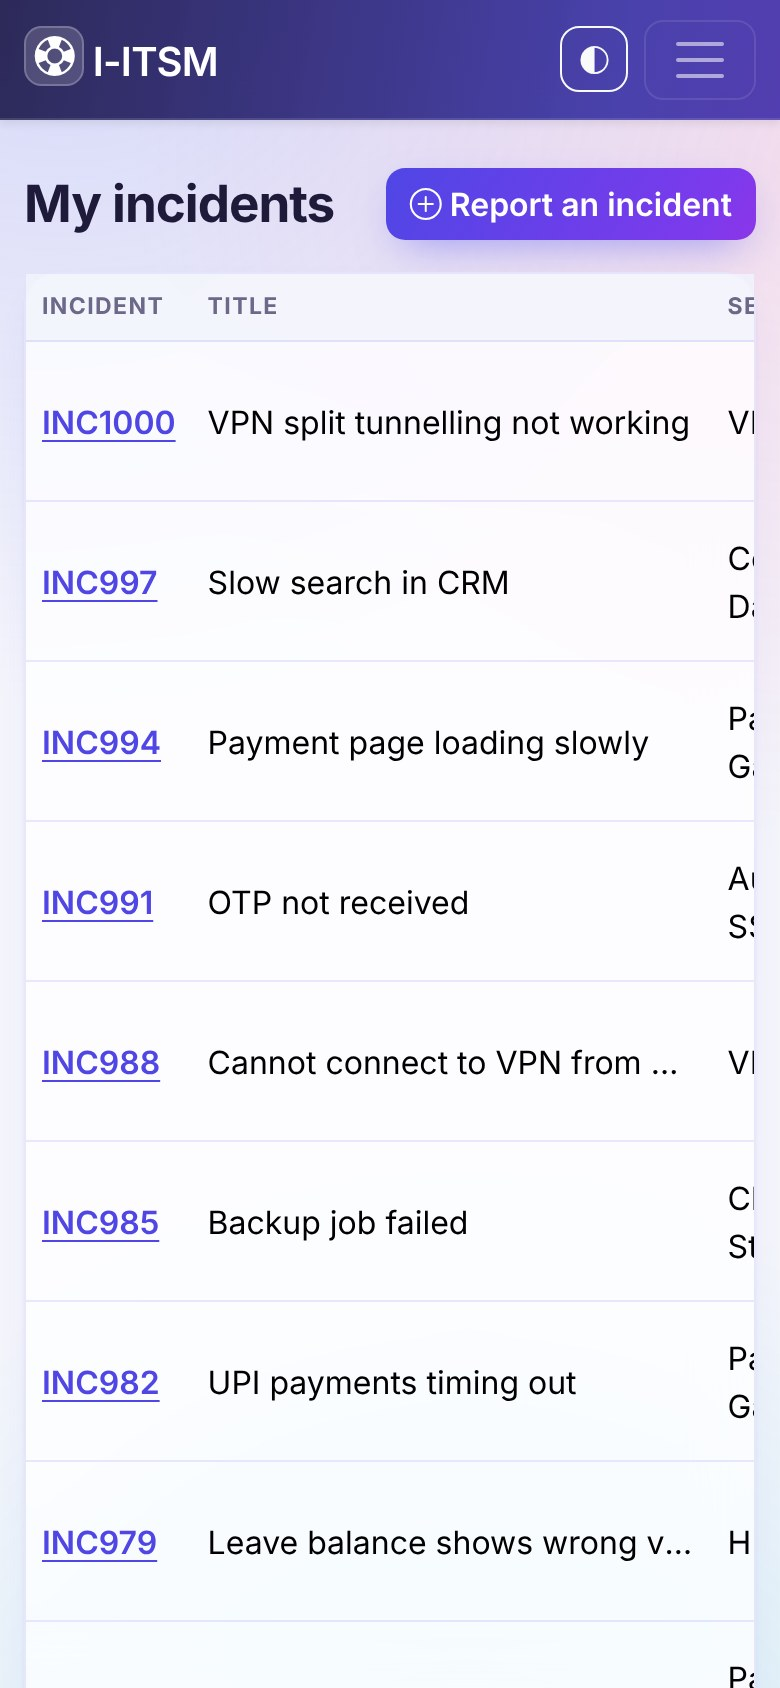
\includegraphics[width=0.92\linewidth]{figures/shot-29-mobile.jpg}\end{minipage}\hfill
\begin{minipage}[c]{0.66\linewidth}
\small The interface adapts to phone width without sideways scrolling: the menu collapses behind a button and tables scroll inside their cards. Colours follow the system's light or dark setting unless the user picks a theme with the button in the top bar; the choice is remembered in the browser. A skip-to-content link, visible focus outlines and the \texttt{/} shortcut for search help keyboard users.
\end{minipage}
\caption{The employee view on a phone (390 pixels wide).}
\end{figure}

\subsection{Technician and team lead}
\begin{enumerate}
  \item \textbf{Work the queue.} \emph{My queue} lists assigned incidents with the most urgent SLA first, and the workload bar shows active incidents against the technician's maximum. The availability switch takes the technician out of automatic assignment (for example, when on leave).
  \item \textbf{Acknowledge, investigate, resolve.} On the incident page: acknowledge (stops escalation and records the response time), start the investigation, add notes, ask the reporter a question, and resolve with a summary and root cause. Suggested resolutions from similar past incidents and the AI advisor help with the diagnosis.
  \item \textbf{Duplicates.} When a report is flagged as a possible duplicate, confirm it (it is linked to the original) or dismiss it.
  \item \textbf{Team leads} additionally see all incidents and the team's workload, and receive the first level of escalation.
\end{enumerate}

\shot{30-dark-tech}{A technician's queue in dark mode.}

\subsection{Administrator}
\begin{itemize}
  \item \textbf{Overview:} incident figures, at-risk and unassigned incidents, technician workload, outage hotspots and charts.
  \item \textbf{Incidents:} all incidents; classify NEW incidents, assign or reassign with the smart recommendation, change impact or urgency (priority and SLA are recalculated).
  \item \textbf{Configure:} users and technicians (skills, maximum workload, experience, team lead, availability), IT services (criticality, dependencies), categories (with keywords for suggestions), SLA policies per service and priority, and the assignment strategy.
  \item \textbf{Monitor:} the audit log (filterable, exportable to CSV) and the e-mail / SMS outbox.
\end{itemize}

\twoshots{16-users}{Users and technicians; administrators create technician and administrator accounts.}{27-technician-profile}{A technician's skills, capacity, experience, team-lead flag and availability.}
\twoshots{26-categories}{Categories are data: new ones are added here, with keywords for suggestion.}{10-admin-incidents}{All incidents with priority, status, SLA and assignee.}
\twoshots{25-forbidden}{Role checks: an employee who opens an administrator page sees a 403 page.}{28-admin-incident-pending}{The administrator's view of an incident: re-assignment with scores and impact changes.}

% ================================================================== 12a
\section{Source Code, Build and Deployment}
The complete source code is in the Git repository \url{\repourl}. It contains 164 main types (about 9,100 lines of Java) in the package \code{com.iitsm}, 27 test classes with 249 tests, 23 page templates, the design decision log (\code{docs/decisions.md}, 26 entries) and the documented test cases.

\subsection{Repository layout}
\begin{tabularx}{\linewidth}{@{}L{5.6cm}Y@{}}
\toprule
\textbf{Path} & \textbf{Contents} \\
\midrule
\code{src/main/java/com/iitsm} & Application code, one package per layer or concern (Appendix~\ref{app:classes}) \\
\code{src/main/resources/\allowbreak templates} & Thymeleaf pages, one folder per role \\
\code{src/main/resources/\allowbreak static} & Stylesheet, script and images of the interface \\
\code{src/main/resources/\allowbreak application*.yml} & Settings: default (H2), \code{dev}, \code{demo} (PostgreSQL) \\
\code{src/test/java} & JUnit 5 tests \\
\code{docs/} & This report and its diagrams, decision log, test cases, plan \\
\code{docker-compose.yml} & PostgreSQL 16 for the demo profile \\
\bottomrule
\end{tabularx}

\subsection{Requirements and commands}
Java 21 (JDK) and Maven 3.9 are required; Docker is needed only for the PostgreSQL profile. The first build downloads the dependencies, including the bundled front-end libraries, after which the application runs offline.

\begin{tabularx}{\linewidth}{@{}L{5.6cm}Y@{}}
\toprule
\textbf{Task} & \textbf{Command} \\
\midrule
Run the tests & \code{mvn test} \\
Run with the in-memory database & \code{mvn spring-boot:run}, then open \code{http://localhost:8080} \\
Run with PostgreSQL & \code{docker compose up -d}, then \code{mvn spring-boot:run -Dspring-boot.run.profiles=demo} \\
Developer profile (H2 console, SQL log) & \code{mvn spring-boot:run -Dspring-boot.run.profiles=dev} \\
Enable the Gemini AI advisor & set the environment variable \code{GEMINI\_API\_KEY} \\
Windows one-click start & \code{run.bat} (uses \code{start-app.ps1}, opens the browser when ready) \\
\bottomrule
\end{tabularx}

\subsection{Configuration}
\begin{tabularx}{\linewidth}{@{}L{6.2cm}Y@{}}
\toprule
\textbf{Setting} & \textbf{Effect} \\
\midrule
\code{itsm.priority.strategy} & \code{weighted} (default) or \code{matrix} \\
\code{itsm.sla.monitor-interval} & How often the SLA monitor runs (default 20 seconds) \\
\code{itsm.sla.risk-threshold} & Fraction of an SLA window after which an incident is at risk (0.75) \\
\code{itsm.duplicates.threshold} & Similarity at which a report is flagged as a duplicate (0.5) \\
\code{itsm.escalation.enabled} & Turns automatic escalation on or off \\
\code{itsm.demo-data.enabled} & Creates demo accounts, services and history on an empty database \\
\code{itsm.notifications.channels.*} & Channels per role (in-app, e-mail, SMS) \\
\bottomrule
\end{tabularx}

% ================================================================== 12
\section{Limitations and Future Work}
\begin{itemize}
  \item The SLA clock does not pause while waiting for the reporter, and there are no business-hours calendars.
  \item Duplicate detection compares words, not meaning; text embeddings could replace it behind the same \code{DuplicateDetector} interface.
  \item E-mail and SMS are simulated; real providers need one adapter class each.
  \item Pages do not update live; WebSocket or server-sent events would be the next step.
  \item Dashboard figures are computed in memory and would move to SQL at large scale.
\end{itemize}

\section{Team Contributions}
The work was divided by module so that every member owns a clearly identifiable part of the system, as the brief requires, while all four members took part in the design discussions, code reviews and testing and can explain the whole system. Each member presents their own module in the demonstration video.

\begin{longtable}{@{}L{3.5cm}L{5.3cm}L{6.4cm}@{}}
\toprule
\textbf{Member} & \textbf{Module and responsibilities} & \textbf{Main classes and artefacts} \\
\midrule\endhead
\textbf{Vijay Srivathsan B}\newline 2024B3A70537H & \textbf{Domain, OOP, database.} Layered architecture; the \code{Incident} aggregate and value objects; the user hierarchy; the State pattern for the lifecycle; factories; the exception hierarchy; persistence, repositories and the database design. & \code{Incident}, \code{User} hierarchy, \code{domain.incident.state}, \code{IncidentFactory}, \code{UserFactory}, \code{ItsmException} family, repositories, ER design \\
\textbf{Sathvik T Hatwar}\newline 2024B3A70509H & \textbf{Priority, SLA, assignment.} Priority strategies and their explanation; SLA policies, deadline tracking, the background SLA monitor and risk detection; technician assignment strategies and the runtime strategy registry. & \code{priority} package, \code{SlaService}, \code{SlaMonitorService}, \code{ThresholdSlaRiskEvaluator}, \code{assignment} package, \code{AssignmentStrategyRegistry} \\
\textbf{Harish MP}\newline 2024B5A70641H & \textbf{UI, security, audit, admin.} Role-specific Thymeleaf pages, theme and accessibility; Spring Security and access control; the audit trail and notifications (Observer, Adapter); administrator screens, dashboard, search and CSV export. & \code{web} package, templates, \code{app.css}, \code{SecurityConfig}, \code{GlobalExceptionHandler}, \code{AuditListener}, \code{NotificationListener}, \code{ReportService}, \code{SearchService} \\
\textbf{Vishnu Rahul}\newline 2024B4AD0542H & \textbf{Intelligent features, tests.} Duplicate detection and correlation, category and resolution suggestions, automatic escalation, the Gemini AI advisor and the service dependency graph; the automated test suite and the documented test cases. & \code{intelligence} package, \code{EscalationService}, \code{AiIncidentAdvisor}, \code{ITService} dependencies, test suite, \code{docs/test-cases.md} \\
\bottomrule
\end{longtable}

\subsection{Demonstration plan}
\begin{tabularx}{\linewidth}{@{}L{3.6cm}L{2.2cm}Y@{}}
\toprule
\textbf{Presenter} & \textbf{Time} & \textbf{Part of the video} \\
\midrule
Vijay Srivathsan B & 0--4 min & Introduction, architecture, domain model, State pattern and database; an illegal transition being rejected. \\
Sathvik T Hatwar & 4--9 min & Workflow 1 (report $\rightarrow$ prioritise $\rightarrow$ assign $\rightarrow$ notify): the priority working, the SLA countdown and risk badge, switching the assignment strategy. \\
Harish MP & 9--13 min & Workflow 2 (investigate $\rightarrow$ resolve $\rightarrow$ verify $\rightarrow$ close) through the role-based pages; access control (403); audit log, notifications and outbox; administrator screens, dashboard, dark mode. \\
Vishnu Rahul & 13--18 min & Workflow 3: duplicate detection, outage hotspot and escalation; AI advisor and dependency impact; the test suite running. \\
\bottomrule
\end{tabularx}

\section{Conclusion}
I-ITSM shows how object-oriented design keeps a realistic system maintainable: each incident status is its own class, each algorithm is a swappable strategy, side effects hang off events, and new categories, strategies or channels are added without editing unrelated code. The application covers every MVP requirement of the brief, implements all seven suggested intelligent features plus three extensions, and is backed by 249 automated tests.

\clearpage
\appendix
\renewcommand{\thesection}{\Alph{section}}
\section{Class Catalogue}\label{app:classes}
Every type in \code{src/main/java}, grouped by package, with the first sentence of its Javadoc as its responsibility. This is the list each member uses to explain any class in the viva.
{\small% generated from the Javadoc of every class in src/main/java (164 types)
\begin{longtable}{@{}L{4.6cm}L{1.9cm}L{8.6cm}@{}}
\toprule
\textbf{Type} & \textbf{Kind} & \textbf{Responsibility} \\
\midrule\endhead
\multicolumn{3}{@{}l}{\cellcolor{rowtint}\textbf{\code{com.iitsm.domain}}} \\
\code{Base\-Entity} & abstract class & Common identity for every persistent entity: a database-generated id, an optimistic-locking version, and id-based equality (two objects are the same entity if they share an id). \\
\code{Checks} & class & Small guard helpers used by domain constructors and methods to protect their invariants. \\
\multicolumn{3}{@{}l}{\cellcolor{rowtint}\textbf{\code{com.iitsm.domain.user}}} \\
\code{Administrator} & class & An administrator / IT manager who configures the system and monitors incidents. \\
\code{Employee} & class & An employee/customer who reports incidents and follows them until they are closed. \\
\code{New\-User} & record & Details common to every new user, passed to UserFactory. The raw password is hashed by the factory and never stored. \\
\code{Role} & enum & Security role of a user. Each User subtype maps to exactly one role. \\
\code{Technician} & class & A support engineer who investigates and resolves incidents. Skills are an aggregation of Category objects: categories exist independently of any technician and are shared between many technicians. \\
\code{User} & abstract class & Anyone who can log in. Abstract because every real user is exactly one of Employee, Technician or Administrator (genuine "is-a" relationships). \\
\code{User\-Factory} & class & Factory pattern: the single place that creates User objects. \\
\multicolumn{3}{@{}l}{\cellcolor{rowtint}\textbf{\code{com.iitsm.domain.incident}}} \\
\code{Feedback} & class & The reporter's rating (1-5) and comment after resolution. An immutable value embedded in the incident row (composition). \\
\code{Impact} & enum & How widely an incident affects the business. The weight feeds the priority calculation. \\
\code{Incident} & class & The central aggregate: one reported IT problem and everything that happens to it. \\
\code{Incident\-Factory} & class & Factory pattern: turns an employee's IncidentReport into a valid NEW Incident. \\
\code{Incident\-Number} & record & Value object for the human-readable incident number shown to users, e.g. INC1001. \\
\code{Incident\-Operation} & enum & The lifecycle operations that can be requested on an incident. \\
\code{Incident\-Report} & record & What an employee fills in when reporting a problem. Passed to IncidentFactory. \\
\code{Incident\-Status} & enum & Persisted lifecycle status of an incident. Which transitions are legal is decided by the State pattern classes in domain.incident.state (Milestone 3), not by this enum. \\
\code{Investigation\-Note} & class & One entry in an incident's investigation log: a technician note, an information request, or the reporter's reply. \\
\code{Note\-Type} & enum & Kind of entry in an incident's conversation/investigation log. \\
\code{Priority} & enum & Incident priority, P1 being the most urgent. Calculated by a PriorityStrategy (Milestone 4). \\
\code{Resolution} & class & How an incident was fixed. An immutable value embedded in the incident row (composition). \\
\code{Urgency} & enum & How quickly the business needs an incident fixed. The weight feeds the priority calculation. \\
\multicolumn{3}{@{}l}{\cellcolor{rowtint}\textbf{\code{com.iitsm.domain.incident.state}}} \\
\code{Abstract\-Incident\-State} & abstract class & Default behaviour for every state: reject every operation. Concrete states override only the operations they allow, so an illegal transition (e.g. NEW $\rightarrow$ CLOSED) can never slip through. \\
\code{Acknowledged\-State} & class & The technician has accepted the incident (the SLA response time is met here). \\
\code{Assigned\-State} & class & A technician has been given the incident but has not acknowledged it yet (escalation watches this state). \\
\code{Classified\-State} & class & Category, priority and SLA are set; waiting for a technician. \\
\code{Closed\-State} & class & Final state. Every operation is rejected. \\
\code{In\-Progress\-State} & class & The technician is investigating. They can ask the reporter for information or resolve it. \\
\code{Incident\-State} & interface & State pattern: one implementation per lifecycle status. Each operation either returns the status the incident moves to, or throws InvalidStateTransitionException if it is not allowed in this state. \\
\code{Incident\-State\-Registry} & class & Maps each persisted IncidentStatus to its IncidentState object. \\
\code{New\-State} & class & Just reported. The only way forward is classification (category, priority, SLA). \\
\code{Pending\-Info\-State} & class & Waiting for the reporter to answer an information request. \\
\code{Resolved\-State} & class & A fix has been provided. The reporter verifies it, or reopens the incident if it is not fixed. \\
\code{Verified\-State} & class & The reporter confirmed the fix. Ready to be closed. \\
\multicolumn{3}{@{}l}{\cellcolor{rowtint}\textbf{\code{com.iitsm.domain.catalog}}} \\
\code{Category} & class & An incident category such as Network or Database. Categories are stored as data rather than a Java enum, so an administrator can add a new one without changing or redeploying code (open-closed principle). \\
\code{ITService} & class & An IT service the organisation runs (Payment Gateway, Email, VPN, ...). \\
\multicolumn{3}{@{}l}{\cellcolor{rowtint}\textbf{\code{com.iitsm.domain.sla}}} \\
\code{Sla\-Policy} & class & Response and resolution targets for one priority, either for a specific service or - when service is null - the default for all services. \\
\code{Sla\-Record} & class & The SLA timings of one incident: deadlines, when they were actually met, and the resulting status. \\
\code{Sla\-Status} & enum & Where an incident stands against its SLA. \\
\multicolumn{3}{@{}l}{\cellcolor{rowtint}\textbf{\code{com.iitsm.domain.audit}}} \\
\code{Audit\-Entry} & class & One immutable line of the audit trail, e.g. "10:07 - INC1024 assigned to tech1 by system". \\
\multicolumn{3}{@{}l}{\cellcolor{rowtint}\textbf{\code{com.iitsm.priority}}} \\
\code{Matrix\-Priority\-Strategy} & class & Alternative algorithm: the classic ITIL impact x urgency matrix. \\
\code{Priority\-Input} & record & Everything a PriorityStrategy may use to decide priority. A small value object, so strategies can be tested without building a whole incident. \\
\code{Priority\-Result} & record & The outcome of a priority calculation: the priority plus a human-readable explanation of how it was reached (shown on the incident page so users can see why it is P1). \\
\code{Priority\-Service} & class & Holds every PriorityStrategy Spring finds and delegates to the one named in itsm.priority.strategy. \\
\code{Priority\-Strategy} & interface & Strategy pattern: an interchangeable algorithm for turning incident facts into a priority. \\
\code{Weighted\-Scoring\-Priority\-Strategy} & class & Default priority algorithm (docs/plan.md section 5): Example: payment outage, HIGH x HIGH x 5 = 45, x 1.5 for 500 users = 67.5 $\rightarrow$ P1. \\
\multicolumn{3}{@{}l}{\cellcolor{rowtint}\textbf{\code{com.iitsm.assignment}}} \\
\code{Assignment\-Service} & class & Everything about who works on an incident: automatic assignment with the active AssignmentStrategy, manual (re)assignment, smart recommendations and workload figures. \\
\code{Assignment\-Strategy} & interface & Strategy pattern: an interchangeable rule for choosing a technician. \\
\code{Assignment\-Strategy\-Registry} & class & Knows every AssignmentStrategy (Spring injects all implementations) and which one is active. \\
\code{Candidate} & record & A technician who could take an incident, together with the numbers a strategy needs. \\
\code{Load\-Based\-Assignment\-Strategy} & class & Spreads work evenly: the technician with the fewest active incidents wins, whatever their skills. \\
\code{Round\-Robin\-Assignment\-Strategy} & class & Takes turns: skilled technicians (or everyone, if nobody has the skill) in a fixed order, starting after whoever got the previous incident of that category. \\
\code{Skill\-Based\-Assignment\-Strategy} & class & Only technicians who have the incident's category as a skill. \\
\code{Smart\-Recommendation\-Strategy} & class & Intelligent feature D - smart technician recommendation. Scores every candidate out of 100: and explains the score, so an administrator can see why someone was recommended. \\
\code{Technician\-Score} & record & One entry in a strategy's ranking: who, how good a match (higher is better) and why. \\
\code{Technician\-Workload} & record & A row of the technician workload report. \\
\multicolumn{3}{@{}l}{\cellcolor{rowtint}\textbf{\code{com.iitsm.sla}}} \\
\code{Default\-Sla\-Policy\-Initializer} & class & On start-up, makes sure the default SLA policies (P1-P4) exist, in every profile. \\
\code{Monitor\-Result} & record & What one SLA monitor run did (for the log and tests). \\
\code{Sla\-Monitor} & class & Background job: runs the SLA checks on a fixed delay (itsm.sla.monitor-interval, default one minute). \\
\code{Sla\-Monitor\-Service} & class & One pass of continuous SLA monitoring (run every minute by SlaMonitor): for every open incident, detect breaches (SLA\_VIOLATED) and SLA risk (SLA\_APPROACHING, feature E), then escalate overdue unacknowledged major incidents (feature C). \\
\code{Sla\-Risk\-Evaluator} & interface & Intelligent feature E - decides whether an incident is likely to miss its SLA, so people are warned before the deadline. \\
\code{Sla\-Service} & class & Finds which SLA policy applies to an incident: the service's own policy for that priority if one exists, otherwise the default policy for the priority. \\
\code{Threshold\-Sla\-Risk\-Evaluator} & class & An incident is AT RISK when 75\% (configurable) of the response window has passed and nobody has acknowledged it, or 75\% of the resolution window has passed, or 50\% of the resolution window has passed and the assigned technician is at least 80\% busy. \\
\multicolumn{3}{@{}l}{\cellcolor{rowtint}\textbf{\code{com.iitsm.event}}} \\
\code{Incident\-Event} & record & Observer pattern: the "subject" (IncidentService, later also the SLA monitor) publishes one of these after every change, and any number of "observers" (audit, notifications, escalation) listen for it. \\
\code{Incident\-Event\-Publisher} & class & The single place that turns "something happened to this incident" into an IncidentEvent and hands it to Spring's event bus. \\
\code{Incident\-Event\-Type} & enum & Everything that can happen to an incident and that other parts of the system may react to (audit, notifications, escalation). \\
\multicolumn{3}{@{}l}{\cellcolor{rowtint}\textbf{\code{com.iitsm.audit}}} \\
\code{Audit\-Listener} & class & Observer: writes one AuditEntry for every IncidentEvent, giving a complete, chronological history (who, what, when, from which status to which). \\
\code{Audit\-Service} & class & Read access to the audit trail: one incident's history, and the recent system-wide log for administrators with simple filters. \\
\multicolumn{3}{@{}l}{\cellcolor{rowtint}\textbf{\code{com.iitsm.notification}}} \\
\code{Audience} & enum & Groups of people who may need to hear about an incident event. \\
\code{Email\-Gateway} & interface & Adapter pattern - the target interface: what I-ITSM needs from an email provider. \\
\code{Email\-Notification\-Channel} & class & Sends the notification through the EmailGateway and records it as a delivery log entry. \\
\code{In\-App\-Notification\-Channel} & class & Stores the notification in the database; the web UI shows it under the bell icon until read. \\
\code{In\-Memory\-Outbox} & class & A bounded, thread-safe list of the most recent outbox messages. \\
\code{Logging\-Email\-Gateway} & class & Simulated email provider (the brief allows simulation): instead of contacting a mail server it writes the message to the log and keeps it in an in-memory outbox that administrators can view. \\
\code{Logging\-Sms\-Gateway} & class & Simulated SMS provider: logs the text (cut to 160 characters, like a real SMS) and keeps it in an in-memory outbox. \\
\code{Notification\-Channel} & interface & Strategy pattern: one way of delivering a notification (in-app, email, SMS, ...). \\
\code{Notification\-Factory} & class & Factory pattern: builds the NotificationMessage for an event, so wording lives in one place and every channel sends the same content. \\
\code{Notification\-Listener} & class & Observer: reacts to every IncidentEvent by deciding who should hear about it (a rule table per event type) and sending the message through each recipient's channels. \\
\code{Notification\-Message} & record & The content of one notification, independent of how it is delivered. \\
\code{Notification\-Preferences} & class & Which channels each role receives, configurable in application.yml, e.g. Defaults: everyone gets in-app and email; technicians and administrators also get SMS for urgent messages. \\
\code{Notification\-Service} & class & The user's in-app inbox (bell icon) and the administrators' view of the simulated email/SMS outbox. \\
\code{Outbox\-Message} & record & A message handed to a (simulated) external gateway, kept so administrators can see what would have been sent by email or SMS. \\
\code{Sms\-Gateway} & interface & Adapter pattern - the target interface for SMS providers (Twilio, MSG91, ...). \\
\code{Sms\-Notification\-Channel} & class & Sends a short text through the SmsGateway - only for urgent messages (major incidents, SLA problems, escalations) and only to users with a phone number. \\
\multicolumn{3}{@{}l}{\cellcolor{rowtint}\textbf{\code{com.iitsm.intelligence}}} \\
\code{Ai\-Incident\-Advisor} & class & Intelligent feature - External AI / Google Gemini API integration for incident triage, automated root-cause analysis, and recommended investigation steps. \\
\code{Category\-Suggester} & class & Intelligent feature F - suggests a category from the incident description by counting how many of each category's keywords (normalised the same way as duplicate detection) appear in the text. \\
\code{Duplicate\-Detection\-Service} & class & Intelligent features A (duplicate detection) and B (incident correlation). \\
\code{Duplicate\-Detector} & interface & Intelligent feature A - how alike a new report is to an existing incident. \\
\code{Duplicate\-Match} & record & An existing incident that looks like the same problem, with its similarity score. \\
\code{Escalation\-Service} & class & Intelligent feature C - automatic escalation. A major (P1/P2) incident that nobody has acknowledged by its response deadline is escalated one level at a time: team lead, then system administrator, then IT manager - one more response window apart. \\
\code{Resolution\-Suggester} & class & Intelligent feature G - finds up to three similar incidents that were already resolved and shows how they were fixed, so a technician can reuse past knowledge. \\
\code{Resolution\-Suggestion} & record & A past incident whose resolution might help with the current one. \\
\code{Text\-Normalizer} & class & Turns free text into a set of meaningful words so two descriptions can be compared: lower-case, punctuation removed, common words ("the", "is", "to", ...) dropped, simple plurals reduced, and synonyms mapped to one word (e.g. "transaction", "checkout" and... \\
\code{Text\-Similarity\-Duplicate\-Detector} & class & Word-overlap (Jaccard) similarity of the normalised title + description, plus a bonus when both incidents are on the same IT service. \\
\multicolumn{3}{@{}l}{\cellcolor{rowtint}\textbf{\code{com.iitsm.service}}} \\
\code{Catalog\-Service} & class & Administration of the service catalogue, incident categories and SLA policies. \\
\code{Dashboard\-Report} & record & Figures for the administrator dashboard, computed by ReportService. \\
\code{Incident\-Action} & enum & Actions a particular user may take on a particular incident right now. \\
\code{Incident\-Search\-Criteria} & record & The search form: every field is optional, and the filters that are filled in are combined with AND. \\
\code{Incident\-Service} & class & Application service for the incident use cases (create, view, update, assign, resolve, close). \\
\code{Report\-Service} & class & Builds the dashboard figures (incident overview, breakdowns per service/category/priority/status, SLA compliance, average resolution time, at-risk incidents and service hotspots). \\
\code{Search\-Service} & class & Multi-criteria incident search. Results are always limited to what the user may see: administrators and team leads see everything, technicians their assigned incidents, employees their own. \\
\code{User\-Service} & class & User management: self-registration of employees, and administrator management of users and technicians (skills, capacity, availability, team-lead flag). \\
\multicolumn{3}{@{}l}{\cellcolor{rowtint}\textbf{\code{com.iitsm.repository}}} \\
\code{Administrator\-Repository} & interface & Repository for administrators (also used to find escalation targets). \\
\code{Audit\-Entry\-Repository} & interface & Repository for the audit trail. \\
\code{Category\-Repository} & interface & Repository for incident categories. \\
\code{Employee\-Repository} & interface & Repository for employees (incident reporters). \\
\code{Escalation\-Repository} & interface & Repository for escalation records. \\
\code{ITService\-Repository} & interface & Repository for the IT service catalogue. \\
\code{Incident\-Repository} & interface & Repository for incidents. JpaSpecificationExecutor enables the multi-criteria search built in Milestone 8. \\
\code{Incident\-Specifications} & class & Small, reusable query conditions (JPA Criteria API) that the search combines with Specification.where(a).and(b)... \\
\code{Notification\-Repository} & interface & Repository for notifications. \\
\code{Sla\-Policy\-Repository} & interface & Repository for SLA policies: service-specific ones and the defaults (service = null). \\
\code{System\-Setting\-Repository} & interface & Repository for runtime settings, keyed by setting name. \\
\code{Technician\-Repository} & interface & Repository for technicians, including the skill lookups used by assignment strategies. \\
\code{User\-Repository} & interface & Repository for all users. Queries are polymorphic: a result can be an Employee, Technician or Administrator object. \\
\multicolumn{3}{@{}l}{\cellcolor{rowtint}\textbf{\code{com.iitsm.web}}} \\
\code{Admin\-Controller} & class & Administrator pages: overview, all incidents, users and technicians, IT services, categories, SLA policies, assignment strategy, audit log and the simulated email/SMS outbox. \\
\code{Auth\-Controller} & class & Login page (the login itself is handled by Spring Security) and employee self-registration. \\
\code{Employee\-Controller} & class & Employee pages: my incidents, and the report form. \\
\code{Global\-Exception\-Handler} & class & Turns exceptions into friendly pages, in one place: not found $\rightarrow$ 404 page; not allowed $\rightarrow$ 403 page; any other business error (invalid transition, invalid input, technician unavailable, ...) $\rightarrow$ back to the page the user came from, with the message shown as... \\
\code{Global\-Model\-Attributes} & class & Adds the logged-in user and their unread-notification count (for the bell icon) to every page. \\
\code{Home\-Controller} & class & Landing page, the role-based "/dashboard" redirect, and the access-denied page. \\
\code{Incident\-Controller} & class & The incident detail page shared by all roles, and every lifecycle action. \\
\code{Notification\-Controller} & class & The in-app notification inbox (behind the bell icon). \\
\code{Search\-Controller} & class & Incident search for every role (results limited to what the user may see). \\
\code{Suggestion\-Api\-Controller} & class & Small JSON endpoint used by the report form to suggest a category while the employee types (feature F). \\
\code{Technician\-Controller} & class & Technician pages: the work queue (most urgent SLA first), workload and availability. \\
\code{View\-Formatter} & class & Formatting helpers for templates, used as \$\{ \\
\multicolumn{3}{@{}l}{\cellcolor{rowtint}\textbf{\code{com.iitsm.web.form}}} \\
\code{Category\-Form} & class & Administrator's form for an incident category. \\
\code{New\-User\-Form} & class & Administrator's form for creating a user of any role. \\
\code{Registration\-Form} & class & Self-registration form (employees only). Validated with Bean Validation before reaching the service. \\
\code{Report\-Incident\-Form} & class & The employee's "report an incident" form. \\
\code{Service\-Form} & class & Administrator's form for an IT service. \\
\code{Sla\-Policy\-Form} & class & Administrator's form for an SLA policy (no service = default policy). \\
\code{Technician\-Form} & class & Administrator's form for a technician's skills and capacity. \\
\multicolumn{3}{@{}l}{\cellcolor{rowtint}\textbf{\code{com.iitsm.security}}} \\
\code{Current\-User\-Provider} & class & Gives controllers the logged-in User entity (freshly loaded, so role-specific fields such as a technician's skills are up to date). \\
\code{Itsm\-User\-Details\-Service} & class & Tells Spring Security how to find a user at login. Password checking (BCrypt) and the "invalid login" response are handled by Spring Security itself. \\
\code{Itsm\-User\-Principal} & class & Adapter between our User entity and Spring Security's UserDetails. \\
\multicolumn{3}{@{}l}{\cellcolor{rowtint}\textbf{\code{com.iitsm.exception}}} \\
\code{Assignment\-Exception} & abstract class & Base class for problems assigning an incident to a technician. \\
\code{Category\-Not\-Found\-Exception} & class & Thrown when an incident category id or name does not exist. \\
\code{Duplicate\-Incident\-Exception} & class & Thrown when an employee reports the same problem again shortly after their own identical report. \\
\code{External\-Service\-Exception} & class & An external system (email server, SMS provider, ...) failed or could not be reached. \\
\code{Incident\-Not\-Found\-Exception} & class & Thrown when no incident has the requested number. \\
\code{Invalid\-Input\-Exception} & class & Thrown when a value violates a domain rule (blank name, out-of-range criticality, bad password, ...). \\
\code{Invalid\-State\-Transition\-Exception} & class & Thrown by the State pattern when an operation is not allowed in the incident's current status, e.g. closing a NEW incident. \\
\code{Itsm\-Exception} & abstract class & Root of the I-ITSM exception hierarchy. All business errors extend this, so one handler can turn any of them into a friendly message. \\
\code{Missing\-Sla\-Configuration\-Exception} & class & Thrown when neither a service-specific nor a default SLA policy exists for a priority. \\
\code{Not\-Found\-Exception} & abstract class & Base class for "the thing you asked for does not exist" errors (shown as HTTP 404). \\
\code{Service\-Not\-Found\-Exception} & class & Thrown when an IT service id or name does not exist. \\
\code{Technician\-Unavailable\-Exception} & class & Thrown when the chosen technician is inactive or marked unavailable, or no technician can take the incident. \\
\code{Unauthorized\-Operation\-Exception} & class & Thrown when a logged-in user tries something their role or relationship to the incident does not allow (HTTP 403). \\
\code{User\-Not\-Found\-Exception} & class & Thrown when a user id or username does not exist. \\
\code{Workload\-Exceeded\-Exception} & class & Thrown when assigning would push a technician over their maximum workload. \\
\multicolumn{3}{@{}l}{\cellcolor{rowtint}\textbf{\code{com.iitsm.config}}} \\
\code{Clock\-Config} & class & Provides the system Clock. Every class that needs "now" asks this clock instead of calling Instant.now() directly, so tests (and the demo) can use a fixed or fast-forwarded clock to check SLA deadlines and escalation. \\
\code{Password\-Config} & class & Password hashing. BCrypt is salted and deliberately slow, so leaked hashes are hard to crack. \\
\code{Scheduling\-Config} & class & Turns on background jobs (the SLA monitor). Disabled in tests with itsm.scheduling.enabled=false, where the monitor is run directly with a controllable clock. \\
\code{Security\-Config} & class & Authentication and role-based access: form login with BCrypt passwords (see PasswordConfig); CSRF protection on for every form; URL rules per role: /employee/**, /tech/**, /admin/**; \\
\multicolumn{3}{@{}l}{\cellcolor{rowtint}\textbf{\code{com.iitsm.bootstrap}}} \\
\code{Demo\-Data\-Loader} & class & Seeds an EMPTY database with the demo accounts (docs/demo-accounts.md), IT services and incident categories so the app can be used straight away. \\
\code{Historical\-Incident\-Seeder} & class & Creates about 30 past incidents (2-20 days old) so dashboards, search, reports and the "suggested resolution" feature have realistic data. \\
\multicolumn{3}{@{}l}{\cellcolor{rowtint}\textbf{\code{com.iitsm}}} \\
\code{Itsm\-Application} & class & Entry point of the I-ITSM application. Spring Boot scans com.iitsm and its sub-packages. \\
\multicolumn{3}{@{}l}{\cellcolor{rowtint}\textbf{\code{com.iitsm.domain.escalation}}} \\
\code{Escalation} & class & Record that an unacknowledged major incident was escalated to someone more senior. \\
\code{Escalation\-Level} & enum & The escalation chain from the brief: Technician $\rightarrow$ Team Lead $\rightarrow$ System Administrator $\rightarrow$ IT Manager. \\
\multicolumn{3}{@{}l}{\cellcolor{rowtint}\textbf{\code{com.iitsm.domain.notification}}} \\
\code{Channel\-Type} & enum & The ways a notification can be delivered. Each value has a matching NotificationChannel implementation (Milestone 6). \\
\code{Notification} & class & A message sent to a user. In-app notifications are shown under the bell icon; email and SMS ones are kept as a delivery log. \\
\multicolumn{3}{@{}l}{\cellcolor{rowtint}\textbf{\code{com.iitsm.domain.settings}}} \\
\code{System\-Setting} & class & A setting an administrator can change while the system runs, stored as a key/value pair (e.g. assignment.strategy = skill). \\
\bottomrule
\end{longtable}
}

\section{Documented Test Cases}\label{app:tests}
All 108 documented test cases, covering normal operations, boundary conditions, invalid inputs, exceptions, authorisation and business rules. Each is implemented as an automated JUnit test and passes.
{\small\begin{longtable}{@{}L{1.0cm}L{1.85cm}L{2.15cm}L{4.05cm}L{5.45cm}@{}}
\toprule
\textbf{ID} & \textbf{Area} & \textbf{Type} & \textbf{Scenario} & \textbf{Expected result} \\
\midrule\endhead
TC01 & Platform & Normal & Application context starts & All beans created, no errors \\
TC02 & Web & Normal & Anonymous GET \code{/} & 200 with "I-ITSM is running" \\
TC03 & Security & Authorization & Anonymous GET \code{/admin} & Redirect (302) to login \\
TC04 & Users & Normal & Factory creates each role & Employee / Technician / Administrator subtype returned \\
TC05 & Security & Business rule & New user's password & Stored as BCrypt hash, never raw \\
TC06 & Users & Invalid input & Password of 5 characters & \code{InvalidInputException} \\
TC07 & Users & Invalid input & Blank or "bad name!" username & \code{InvalidInputException} \\
TC08 & Users & Boundary & Technician experience level 6 (max 5) & \code{InvalidInputException} \\
TC09 & Incidents & Normal & Create incident & Status NEW, number INC1001, SLA NOT\_STARTED \\
TC10 & Incidents & Invalid input & Blank title / no service / 0 affected users & \code{InvalidInputException} \\
TC11 & Incidents & Business rule & Modify notes list from outside & \code{UnsupportedOperationException} (encapsulation) \\
TC12 & Catalog & Boundary & Service criticality 0, 1, 5, 6 & 1 and 5 accepted, 0 and 6 rejected \\
TC13 & Assignment & Boundary & Technician at 2/3 vs 3/3 workload & Has capacity at 2, not at 3 \\
TC14 & SLA & Invalid input & Response 0 min, or resolution shorter than response & \code{InvalidInputException} \\
TC15 & Feedback & Boundary & Rating 0, 1, 5, 6 & 1 and 5 accepted, 0 and 6 rejected \\
TC16 & Persistence & Normal & Save incident with a note, reload & All fields and the note come back \\
TC17 & Persistence & Normal & Find technicians by skill & Only active technicians with that skill \\
TC18 & Persistence & Normal & Look up user by username & Returns the right subtype (polymorphic query) \\
TC19 & SLA & Normal & Service-specific vs default SLA policy & Specific found for service, default otherwise, none for missing \\
TC20 & Lifecycle & Business rule & Every (status, operation) pair: 9 statuses x 10 operations & 14 legal pairs reach the planned status; the other 76 throw \code{InvalidStateTransitionException} \\
TC21 & Lifecycle & Exception & Close a NEW incident & \code{InvalidStateTransitionException}: "Cannot close an incident that is NEW" \\
TC22 & Lifecycle & Normal & Report $\rightarrow$ classify $\rightarrow$ assign $\rightarrow$ acknowledge $\rightarrow$ start $\rightarrow$ request/provide info $\rightarrow$ resolve $\rightarrow$ verify $\rightarrow$ close & Ends CLOSED with resolution, feedback, notes \\
TC23 & Lifecycle & Business rule & Illegal operation on a NEW incident & Exception thrown and no field changed \\
TC24 & Lifecycle & Business rule & Reporter reopens a resolved incident & Back IN\_PROGRESS, old resolution cleared, reason logged \\
TC25 & Incidents & Normal & Two employees report incidents & INC1001 and INC1002 created as NEW; CREATED events published \\
TC26 & Authorization & Authorization & Technician tries to report an incident & \code{UnauthorizedOperationException} \\
TC27 & Observer & Normal & Full lifecycle through the service & One event per step, in order, with previous and new status \\
TC28 & Authorization & Authorization & Employee tries to resolve & \code{UnauthorizedOperationException} \\
TC29 & Authorization & Authorization & Technician acknowledges someone else's incident & \code{UnauthorizedOperationException} \\
TC30 & Authorization & Authorization & Employee views another employee's incident & Rejected; reporter and admin can view \\
TC31 & Assignment & Exception & Assign to an unavailable technician & \code{TechnicianUnavailableException} \\
TC32 & Assignment & Boundary & Assign to a technician already at max workload (1/1) & \code{WorkloadExceededException} \\
TC33 & Incidents & Exception & View INC9999 (does not exist) & \code{IncidentNotFoundException} \\
TC34 & Priority & Business rule & Plan examples: payment outage, VPN, email, HR portal & P1, P2, P3, P4 \\
TC35 & Priority & Boundary & Scores 30 / 29.9 / 15 / 14.9 / 6 / 5.9 & P1 / P2 / P2 / P3 / P3 / P4 \\
TC36 & Priority & Boundary & Affected users 9 / 10 / 99 / 100 / 999 / 1000 & Factor 1.0 / 1.2 / 1.2 / 1.5 / 1.5 / 2.0 \\
TC37 & Priority & Normal & All 9 impact $\times$ urgency combinations (matrix strategy) & Matches the ITIL matrix \\
TC38 & Priority & Business rule & Same input, two strategies & Weighted gives P1, matrix gives P3 (interchangeable algorithms) \\
TC39 & Priority & Invalid input & Configured strategy name "magic" & Start-up fails with a clear message \\
TC40 & SLA & Boundary & Response exactly at the 5-minute deadline & Not a breach (ON\_TRACK) \\
TC41 & SLA & Boundary & Response 1 second after the deadline & BREACHED \\
TC42 & SLA & Business rule & Late response, then resolved in time & Stays BREACHED (breach is permanent) \\
TC43 & SLA & Business rule & Deadline passes, checked repeatedly & Breach reported only once \\
TC44 & Classification & Normal & Employee reports with a category & Auto-classified P1, deadlines +5 min / +30 min, CLASSIFIED event by "system" \\
TC45 & SLA & Exception & Classify with no SLA policy configured & \code{MissingSlaConfigurationException} \\
TC46 & Priority & Normal & Reporter lowers impact and urgency to LOW & Priority P3, new 8 h deadline, PRIORITY\_CHANGED event \\
TC47 & SLA & Exception & Technician acknowledges 6 minutes after a P1 is reported & SLA BREACHED, SLA\_VIOLATED event published \\
TC48 & SLA & Normal & Resolved 20 minutes into a 30-minute window & SLA MET \\
TC49 & Assignment & Normal & Skill-based: two database technicians and one network technician & Only database technicians, least busy first \\
TC50 & Assignment & Boundary & Skill-based: two technicians with equal workload & The more experienced one wins \\
TC51 & Assignment & Normal & Load-based & Least busy first, skills ignored (priority-queue order) \\
TC52 & Assignment & Normal & Round-robin, three incidents & Turns rotate alice $\rightarrow$ bob $\rightarrow$ alice among skilled technicians \\
TC53 & Intelligence (D) & Business rule & Smart recommendation & Skilled senior with service history scores 90 and ranks first; the reason explains the score \\
TC54 & Assignment & Boundary & Any strategy with no candidates & Nobody selected \\
TC55 & Assignment & Normal & Employee reports a database incident & Auto-assigned to the database technician; CREATED $\rightarrow$ CLASSIFIED $\rightarrow$ ASSIGNED events \\
TC56 & Assignment & Exception & Only skilled technician is at max workload & Incident stays CLASSIFIED; NO\_TECHNICIAN\_AVAILABLE event \\
TC57 & Assignment & Business rule & Admin switches strategy from skill to load & Next incident goes to the least busy technician; choice persisted \\
TC58 & Authorization & Invalid input & Unknown strategy name / employee changes strategy & \code{InvalidInputException} / \code{UnauthorizedOperationException} \\
TC59 & Assignment & Business rule & Technician marked unavailable & Never a candidate \\
TC60 & Audit & Normal & Full lifecycle of a P1 incident & 8 audit lines in order with actor (emp1 / system / tech1), previous and new status, timestamps \\
TC61 & Audit & Normal & Admin filters audit log by actor and by action + incident & Only matching lines returned \\
TC62 & Authorization & Authorization & Employee reads the system-wide audit log & \code{UnauthorizedOperationException} \\
TC63 & Notification & Normal & P1 incident auto-assigned & Technician gets in-app, email and SMS; gateway outboxes show the email and SMS \\
TC64 & Notification & Business rule & P4 incident assigned & In-app only, no SMS (not urgent) \\
TC65 & Notification & Business rule & Employee with a phone number & Never receives SMS (role preferences) \\
TC66 & Notification & Business rule & Technician acknowledges & Reporter notified; technician not notified of their own action \\
TC67 & Notification & Exception & No technician available for a P1 & Administrators alerted (in-app + SMS) \\
TC68 & Authorization & Authorization & Marking someone else's notification read / non-admin viewing the outbox & \code{UnauthorizedOperationException} \\
TC69 & Notification & Exception & SMS provider unreachable & Incident still created and assigned; in-app and email still delivered \\
TC70 & Security & Authorization & Anonymous user opens /employee & Redirected to the login page \\
TC71 & Security & Invalid input & Log in with a wrong password & Redirect to /login?error \\
TC72 & Security & Normal & Log in as emp1 & Redirect to /dashboard, then to /employee \\
TC73 & Authorization & Authorization & Employee opens /admin; technician opens /employee/report & 403 \\
TC74 & Web & Normal & Admin opens all 9 admin pages & All render (200) \\
TC75 & Web & Normal & Employee submits a valid report form & Redirect to the new incident page with a success message \\
TC76 & Web & Invalid input & Report form with no service, blank description, 0 users & Form shown again with field errors; nothing saved \\
TC77 & Security & Exception & Form POST without a CSRF token & 403 \\
TC78 & Users & Normal / Invalid input & Register a new employee; register with a taken username & Account created as EMPLOYEE; duplicate refused with an error \\
TC79 & Authorization & Authorization & tech2 resolves tech1's incident; emp2 views emp1's incident & 403 \\
TC80 & Lifecycle & Exception & Technician resolves an ASSIGNED (not started) incident via the UI & Back on the incident page with "Cannot resolve an incident that is ASSIGNED" \\
TC81 & Authorization & Business rule & Actions shown for technician / reporter / admin / other employee & Each sees only what they may do; the other employee sees nothing \\
TC82 & Intelligence (A) & Normal & Text normalisation of the brief's examples & Stopwords dropped; transaction/checkout $\rightarrow$ payment; unavailable/failing/unable $\rightarrow$ outage \\
TC83 & Intelligence (A) & Normal & Three employees report the payment problem in different words & 2nd and 3rd flagged as possible duplicates of the original INC1001; correlated on the service \\
TC84 & Intelligence (A) & Normal & Unrelated VPN report & Not flagged \\
TC85 & Intelligence (A) & Exception & Same employee repeats the same report after 10 minutes & \code{DuplicateIncidentException} naming INC1001 \\
TC86 & Intelligence (A) & Boundary & Same employee repeats it after 61 minutes & Accepted as INC1002 \\
TC87 & Authorization & Authorization & Employee vs assigned technician confirming a duplicate & Employee refused; technician links the incidents \\
TC88 & Intelligence (E) & Boundary & P1 at 73\% / 77\% / 80\% of its window, then past the deadline & Warning at 77\% only, once; breach reported once \\
TC89 & Intelligence (E) & Boundary & P3 at 74.8\% vs 75\%; 50\% with technician 3/5 vs 4/5 busy & At risk at 75\%, or at 50\% when 80\% busy \\
TC90 & Intelligence (C) & Normal & Unacknowledged P1 at 5, 6, 8, 11, 16, 30 min & Escalated to lead1 (6), sysadmin (11), admin (16); nothing at 5, 8, 30; targets notified \\
TC91 & Intelligence (C) & Business rule & Technician acknowledges after the first escalation & No further escalations \\
TC92 & Intelligence (C) & Business rule & P4 left for 24 hours & Never escalated \\
TC93 & Search & Normal & Each of the 10 filters on its own (incl. date boundaries) & Only matching incidents \\
TC94 & Search & Normal & Category + status combined & AND of both filters \\
TC95 & Authorization & Authorization & Search as employee / technician / team lead & Own / assigned / all incidents only \\
TC96 & Reports & Normal & Dashboard figures for 3 incidents & Totals, P1 open, 100\% SLA compliance, 30 min average fix, breakdowns, unassigned list \\
TC97 & Intelligence (C) & Business rule & Overdue P1 assigned to the only team lead & Level 1 skipped; escalated straight to the system administrator \\
TC98 & Intelligence (F) & Normal / Boundary & Suggest a category for "VPN keeps dropping", "cannot complete payment", unrelated text, empty text & NETWORK, APPLICATION, none, none \\
TC99 & Intelligence (G) & Normal & New payment timeout after a resolved UPI timeout; unrelated VPN incident & Past fix suggested for the first; nothing for the second \\
TC100 & Demo data & Normal & Fresh start-up & 9 users, $\geq$25 past incidents (closed on time, closed late, open overdue), all numbered below INC1001, audit history present \\
TC101 & Demo data & Business rule & Loader runs again on a populated database & Nothing added (idempotent) \\
TC102 & Catalog & Normal / Graph & Service dependency graph traversal: add/remove dependencies and check self-dependency guard & Upstream dependencies set, self-dependency prevented \\
TC103 & Intelligence (AI) & Normal / Fallback & AI Incident Advisor triage \& root cause analysis with unconfigured API key & Local heuristic generates triage summary, investigation steps \& root-cause hypothesis \\
TC104 & Web / Export & Normal & Admin exports audit trail to CSV format (\code{/admin/audit/export}) & Status 200, Content-Type \code{text/csv}, Content-Disposition attachment \code{audit-log.csv} \\
TC105 & Web / Export & Normal & User exports search results to CSV format (\code{/search/export}) & Status 200, Content-Type \code{text/csv}, Content-Disposition attachment \code{incidents-export.csv} \\
TC106 & Intelligence (AI) & Boundary & AI Incident Advisor on a NEW (unclassified) incident with no priority yet & Advice is produced and says the incident is not yet prioritised; no NullPointerException (incident page renders) \\
TC107 & Web / UI & Normal & Load Bootstrap, Chart.js and \code{app.js} without logging in & Status 200 for each: assets are served by the app (no CDN needed) and are public \\
TC108 & Web / UI & Normal & Open the login page & Page offers the light/dark theme switcher and links no CDN assets \\
\bottomrule
\end{longtable}
}

\section{Design Decision Log}\label{app:decisions}
Notable design decisions, with the alternatives considered and the reasons, from \code{docs/decisions.md}.
{\small\begin{longtable}{@{}L{0.9cm}L{4.3cm}L{10cm}@{}}
\toprule
\textbf{No.} & \textbf{Decision} & \textbf{Alternatives and reasoning} \\
\midrule\endhead
D1 & Java 21 + Spring Boot 3 & Alternatives: Node/Express, Django, plain Java Swing. Why: course is OOP in Java; Spring's DI makes Strategy/Observer/Repository natural and swappable; mature security + JPA; industry-relevant. \\
D2 & Server-rendered Thymeleaf UI (not React SPA) & Alternatives: React + REST. Why: one codebase/language for a short timeline; role-specific views easy with Spring Security; REST endpoints can still be added for intelligent features. Limitation: less dynamic UI. \\
D3 & PostgreSQL (prod/demo) + H2 (tests) & Alternatives: MySQL, MongoDB. Why: relational data (users, incidents, SLAs, audit) with strong integrity; JPA keeps the code DB-agnostic so tests run fast in-memory. \\
D4 & SINGLE\_TABLE inheritance for the User hierarchy & Alternatives: JOINED, TABLE\_PER\_CLASS, a single User class with a role field. Why: Employee/Technician/Administrator are genuine is-a subtypes with only a few extra columns each. One table makes login a single query with no joins and keeps the JPA mapping simple. Trade-off: subtype-only columns must be nullable. \\
D5 & Stateless State objects mapped from a persisted status enum & Alternatives: storing state objects directly, a big switch on status in Incident. Why: JPA persists the simple \code{IncidentStatus} enum, and \code{IncidentStateRegistry} (an \code{EnumMap}) maps it to one shared, stateless \code{IncidentState} object. Each state overrides only the transitions it allows, so adding a state touches one class plus the registry, and illegal transitions fail in one place (\code{AbstractIncidentState}). \\
D6 & A shared \code{BaseEntity} superclass for identity & Alternatives: repeat \code{id}, \code{version}, \code{equals}/\code{hashCode} in every entity. Why: every entity genuinely \textit{is a} persistent, identifiable object, so this is an is-a relationship, not inheritance just to reuse code. One place defines id-based equality (safe for Hibernate proxies) and optimistic locking (\code{@Version}), so two admins editing the same incident can't silently overwrite each other. It's a \code{@MappedSuperclass}, so there's no extra table. \\
D7 & Subtype-only user fields use wrapper types (\code{Integer}, \code{Boolean}) & Because of SINGLE\_TABLE (D4), a Technician's columns are NULL for Employee rows. Wrapper types accept NULL, and the getters translate NULL into safe defaults, so callers never see nulls. \\
D8 & Value objects for incident number, SLA record, resolution and feedback & \code{IncidentNumber} is a record (\code{INC1001}), so user-facing numbers never expose database ids. \code{SlaRecord}, \code{Resolution} and \code{Feedback} are \code{@Embeddable}: they're stored in the incident row and have no identity of their own, which is exactly composition in UML. \\
D9 & Who decides what in the incident lifecycle & \textbf{State objects} decide \textit{whether} an operation is legal in the current status and \textit{which} status comes next. They hold no data and never touch the incident's fields. **\code{Incident}\textbf{ asks its state first, then updates its own fields. If the state rejects the operation, nothing has been changed yet. }\code{IncidentService}\textit{* decides }who* may do it (reporter, assigned technician, administrator) and publishes an event afterwards. Alternatives: one big \code{switch} on status inside \code{Incident}, or states that change the... \\
D10 & Domain events via Spring's \code{ApplicationEventPublisher} (Observer) & Alternatives: a hand-written listener list inside \code{IncidentService}, or calling audit and notification code directly. Why: Spring already provides a well-tested publish/subscribe mechanism. \code{IncidentService} only publishes an immutable \code{IncidentEvent} and doesn't know who listens, so audit (M6), notifications (M6) and escalation (M8) can be added without changing it. \\
D11 & Priority as a Strategy, selected by configuration & Alternatives: one hard-coded formula inside \code{IncidentService}. Why: the brief explicitly allows teams to choose their own algorithm. \code{WeightedScoringPriorityStrategy} (default) and \code{MatrixPriorityStrategy} (ITIL matrix) share one interface, and \code{PriorityService} picks the one named in \code{itsm.priority.strategy}. A new algorithm, such as one based on historical data, is one new \code{@Component}. Every result carries an explanation string, so users can see why an incident is P1. \\
D12 & SLA rules live in \code{SlaRecord}; \code{Incident} drives them & Alternatives: a separate service that edits SLA fields from outside. Why: SLA timing is part of the incident's own state. \code{Incident.acknowledge()} records the response time and \code{Incident.resolve()} records the resolution time automatically, so no caller can forget. \code{SlaService} only chooses \textit{which} policy applies (the service's own, else the default). The rules: meeting a deadline exactly on time is not a breach, a breach is permanent, and it is reported only once. Known limitation: the SLA clock keeps running... \\
D13 & Classification happens automatically when the reporter picks a category & If the employee chooses a category when reporting, the system classifies the incident at once (priority calculated, SLA started), and the audit trail records the actor as \code{system}. Otherwise it stays NEW until an administrator picks a category. Either way the priority is always calculated, never typed in by hand. \\
D14 & Assignment strategies switchable at runtime, stored as a setting & Alternatives: a config-file choice (as for priority), or an \code{if/else} per strategy in the service. Why: the brief asks that the assignment strategy can be changed without redesigning the application, and an administrator should be able to do it from the UI. \code{AssignmentStrategyRegistry} receives every \code{AssignmentStrategy} from Spring and stores the active name in the \code{system\_setting} table, so the choice takes effect immediately and survives restarts. The four strategies are skill, load, round-robin and smart.... \\
D15 & Build output kept out of iCloud (\code{target.nosync}) & The project sits in \code{\textasciitilde{}/Documents}, which is synced by iCloud Drive. iCloud created duplicate files such as \code{UserFactory 2.class} in \code{target/} and offloaded others mid-build, which broke the tests with "Operation timed out". Maven now builds into \code{target.nosync/}, and iCloud does not sync folders whose names end in \code{.nosync}. Moving the whole project outside \code{\textasciitilde{}/Documents} would be safer still. \\
D16 & Audit and notifications are Observers, run in the same transaction & \code{AuditListener} and \code{NotificationListener} are Spring \code{@EventListener}s on \code{IncidentEvent}. They run synchronously, inside the transaction that changed the incident. \textbf{Audit:} an incident change and its audit line commit together or not at all, so the trail can never miss a change. \code{@Order} makes audit run before notifications. \textbf{Notifications:} every channel call is wrapped in try/catch, so a failing email or SMS provider is logged and skipped. It never rolls back the incident change or blocks the other... \\
D17 & Notification design: Strategy (channels) + Adapter (gateways) + Factory (messages) + rule table (recipients) & **\code{NotificationChannel}** (Strategy): in-app, email and SMS share one interface. Each channel decides in \code{accepts()} whether it applies; for example, SMS is used only for urgent messages to users with a phone number. **\code{EmailGateway} / \code{SmsGateway}** (Adapter targets): the channels depend only on these interfaces. The \code{Logging...Gateway} classes simulate a provider and keep an outbox for administrators. A real provider means one new adapter class. **\code{NotificationFactory}** (Factory): builds the message text per... \\
D18 & Web layer: three lines of security, thin controllers, open-session-in-view & \textbf{Security in depth:} 1. URL rules per role in \code{SecurityConfig} (\code{/employee/**}, \code{/tech/**}, \code{/admin/**}). 2. \code{@PreAuthorize("hasRole('ADMIN')")} on administration service methods. 3. Ownership checks in \code{IncidentService} (own incident, assigned incident). Passwords use BCrypt, CSRF protection is on for every form, Bean Validation guards all input, and the H2 console is reachable only in the \code{dev} profile. Invalid logins go to \code{/login?error}; inactive accounts cannot log in. \textbf{Thin controllers:} each action... \\
D19 & Search with JPA Specifications & Each filter is a small \code{Specification\textless{}Incident\textgreater{}} in \code{IncidentSpecifications}. It returns null when its form field is empty, so \code{Specification.allOf(...)} combines only the filters actually used. The search supports 10 criteria (number, text, from, to, status, priority, category, service, technician, SLA status) plus a visibility scope per role. Alternatives: one repository method per combination, which explodes in number, or hand-built JPQL strings, which are error-prone and open to injection. \\
D20 & Intelligent features A, B, C and E, all behind interfaces & \textbf{A, duplicates:} \code{TextNormalizer} handles stopwords, simple plurals and synonyms (transaction/checkout/pay $\rightarrow$ payment; down/failing/unable $\rightarrow$ outage). \code{TextSimilarityDuplicateDetector} scores Jaccard word overlap, +0.2 when the service is the same, and flags a match at 0.5 or above. A match always points at the \textit{original} report, not at another copy. The same employee repeating the same report within an hour gets \code{DuplicateIncidentException}. A person confirms or dismisses each suggestion; the system never... \\
D21 & Demo data drives the real domain model & \code{HistoricalIncidentSeeder} creates its 28 past incidents through the same constructors, \code{PriorityService}, \code{SlaService} and State-pattern methods as live incidents, just with past timestamps. Seeded data therefore always follows the business rules, and the dashboards, search and feature G work from the very first start. The history is numbered below INC1001 and is at least 2 days old, so it never interferes with the live demo (duplicate detection only looks back 24 h). For the video, a Payment Gateway P1... \\
D22 & Chart.js visual analytics on the Admin Dashboard & Alternatives: Server-rendered SVG charts, text-only tables, external Grafana dashboard. Why: Chart.js runs client-side with a single lightweight script (pinned to 4.4.1 and served from a WebJar, see D26) and renders beautiful responsive HTML5 canvases for priority breakdown (doughnut chart) and service distribution (bar chart). It reads the data already prepared by \code{ReportService} and directly fulfills the "Real-time operational dashboard, Analytics and visualization" innovation challenge without backend overhead. \\
D23 & Service dependency graph via self-referencing @ManyToMany & Alternatives: Flat services list, separate dependency table with string foreign keys. Why: Demonstrates OOP aggregation and graph traversal. \code{ITService} defines a self-referencing \code{@ManyToMany} set \code{dependencies} mapped to \code{service\_dependencies}. Calling \code{findByDependenciesContaining()} navigates the graph in reverse to find downstream services impacted by an outage, giving technicians and admins instant impact analysis when investigating incidents. \\
D24 & RFC-4180 compliant CSV export for audit logs and search results & Alternatives: Third-party Apache POI / OpenCSV library. Why: Built with zero external dependencies using Java string builders and HTTP streaming headers (\code{Content-Disposition: attachment}). Escapes quotes and commas according to RFC-4180. Lets administrators export historical audit compliance logs and custom incident query results directly to spreadsheets. \\
D25 & External AI Incident Advisor with Google Gemini API \& local heuristic fallback & Alternatives: Hard-coded advice text or external Python AI microservice. Why: Directly satisfies the evaluation rubric's requirement for "use of APIs (Google API, any other), integration with third-party services". Uses Java 21's native \code{HttpClient} with non-blocking timeout handling. When \code{GEMINI\_API\_KEY} is provided, it calls Google's \code{generateContent} REST endpoint for automated triage and root-cause hypothesis; when offline or unconfigured, it seamlessly falls back to a deterministic rule-based expert... \\
D26 & Dark mode with CSS colour tokens; front-end libraries as WebJars & Alternatives: a second stylesheet for dark mode; keep loading Bootstrap and Chart.js from a CDN. Why: Bootstrap 5.3 switches its own components with \code{data-bs-theme}, so our \code{app.css} only defines colour tokens once per theme and every badge, chart and timeline uses the tokens. The choice (light / dark / system) is stored in the browser and applied by a tiny inline script before the first paint, so there is no white flash. WebJars put the libraries in \code{pom.xml} with exact versions and serve them from the app, so... \\
\bottomrule
\end{longtable}
}

\end{document}
